\part{Background}
\begin{refsection}

\chapter{Introduction}

The importance of non-bonding interactions in our world simply cannot be overstated.
While we may think of the more familiar covalent and ionic bonds as the core of chemistry, more often than not it is non-bonding interactions that dictate the nature of substances, from bulk properties such as tensile strength, to microscopic phenomena like protein-ligand interactions.

At a fundamental level, all non-bonding interactions (indeed, conventional bonding too) are attributable to the electrostatic force.
However, it is more convenient to broadly categorise interactions based on strength and structural motifs that are common to each class.
Such classes include dispersion forces, dipole-dipole interactions, and hydrogen bonding (H-bonding).
In the 19th century, it became apparent that these classes paint an incomplete picture of intermolecular bonding.
As part of their investigation into solvent effects on the colour of iodine solutions in 1949, Bensei and Hildebrand invoked the concept of ``charge-transfer'' complexes to explain the association of molecular iodine with nucleophililc solvent molecules.\autocite{Benesi1949}
Although the electrophilic nature of molecular halogens was already well appreciated with respect to reactivity, this appears to be the first acknowledgement that this understanding could be applied to ground state complexes.
In support of this, Hassel and Hvoslef elucidated the structure of a 1:1 complex of molecular bromine and 1,4-dioxane in 1954, and observed an unusally strong interaction between the two molecules.\autocite{Hassel1954}
The crystal was comprised of long chains of monomers (\cref{fig:hassel-xray}), exhibiting a very short O\dots Br contact (2.71\AA, the sum of the van der Waals (VDW) radii is 3.37\AA), and a slightly lengthened Br--Br bond (2.31\AA~vs 2.28\AA~in gaseous bromine).

\begin{figure}[ht]
  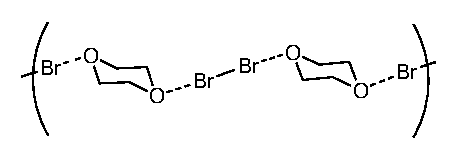
\includegraphics[width=0.6\columnwidth]{Figures/hassel-xray.eps}
  \caption[Bromine-dioxane complex.]{Long chains of molecular bromine and 1,4-dioxane, observed by Hassel and Hvoslef.}
  \label{fig:hassel-xray}
\end{figure}

In the subsequent years, a wide variety of names and labels were applied to the ``charge-transfer'' phenomenon, including ``lock and key'', ``donor-acceptor'', and ``filling of antibonding orbitals'', as summarised in Bent's excellent 1968 review\autocite{Bent1968}.
The term ``halogen bonding'' (X-bonding) only gained widespread acceptance in 1983 after the publication of the review of Dumas, Gomel, and Guerin.\autocite{Dumas1983}
The term deliberately evokes similarity to the better known concept of hydrogen bonding, as the two phenomena are of comparable strength and, importantly, directionality.
In 1998 Anthony C. Legon again used the term to describe the attractive interaction between halogens and Lewis bases in prereactive complexes, harking back to the original understanding of electrophilic halogens as a primarily reactive phenomenon.\autocite{Legon1998,Legon1999}
In the following years, the potential of X-bonding was more fully recognised, with applications in supramolecular chemistry and self-assembly\autocite{Corradi2000,Metrangolo2008,Priimagi2013}, catalysis and bond activation\autocite{Walter2011,Soloshonok2017,Takagi2017}, and molecular sensing and recognition\autocite{Cornes2017,VargasJentzsch2013,Borissov2017}.

From X-bonding grew the related concepts of chalcogen (Ch-), pnicogen (Pn-), and tetrel bonding (T-bonding), as the electrophilic nature of these elements was discovered.\autocite{Murray2007}
Similar applications have also been found for these classes of noncovalent interactions, Ch-bonding in particular.\autocite{Fanfrlik2014,Garrett2016,Ho2016,Wonner2017,Mitchell2017,Benz2017,Biot2018,Ho2017}

\section{Chalcogen Bonding}
Ch-bonding is the attractive interaction between a Lewis base and a chalcogen atom bearing an electron withdrawing substituent (\cref{fig:ch-bonding-intro}).
The terminology of Ch-bonding partners is perhaps counterintuitive, as donors and acceptors are named by analogy with H-bonded equivalents.
Note this is contrary to the formal flow of electron density; Ch-bond \emph{donors} bear vacant \emph{acceptor} orbitals, while Ch-bond \emph{acceptors} are \emph{donors} of electron density.
For the purposes of this thesis, ``donor'' will refer to the Lewis acidic chalcogen species.

\begin{figure}
    \centering
    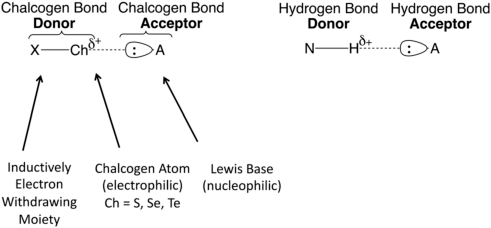
\includegraphics[width=0.8\linewidth]{Figures/ch-bonding.pdf}
    \caption{Chalcogen bonding model, and similarity to H-bonding.}
    \label{fig:ch-bonding-intro}
\end{figure}

\subsection{Mechanisms}
As was discussed in the previous section, all intermolecular (and indeed \emph{intra}molecular) forces are manifestations of the electromagnetic force.
Nonetheless, it is more convenient to categorise energetic contributions to any given interaction as orbital, electrostatic, or dispersion mediated, as there are marked differences in strength and directionality between them.
Historically, X- and Ch-bond interactions were understood to be primarily due to orbital overlap and resulting charge transfer.
Evidence for this included the lengthening of the X--X bond corresponding to increased occupation of the $\sigma^{\star}$(X-X) orbital due to the incoming lone pair (this was observed in Hassel and Hvoslef's original work\autocite{Hassel1954}).
Characteristic charge transfer bands are also observed in the UV-vis spectra of halogen solutions.\autocite{Blackstock1987}

Such evidence of orbital contributions is not, however, common to all systems displaying X- or Ch-bond interactions.
The iodoperfluoroalkanes and arenes studied by Resnati et al. show no charge transfer bands in UV-vis spectra, yet are exceptionally strong X-bond donors.\autocite{Yan2014}
Jane Murray and Peter Politzer have advocated for an alternative, primarily electrostatic explanation of X- and Ch-bond interactions.\autocite{Murray2008,Murray2009}
They propose that a positively charged $\sigma$-hole is generated along the extension of a $\sigma$ bond to an electron withdrawing substituent, due to polarisation of the bonding orbital.
This also adequately explains the strength and directionality of these interactions.
An interpretation which has not attracted as much attention is that of dispersion forces.

While the varying contributions from each of these factors can be dissected computationally via pertubation methods, experimental evidence is surprisingly sparse.
Pascoe, Ling and Cockroft, however, devised an elegant experiment to quantitatively determine energetic contributions.\autocite{Pascoe2017}
\textsuperscript{19}F NMR was used to determine the relative populations of two conformors of a "molecular balance", one bearing a Ch-bond interaction, one not (\cref{fig:cockroft-balances}).
Interaction energies were thus derived, and found to be more or less invariant with respect to the solvent.
This appeared to rule out electrostatic contributions, as solvent dipole moment and bulk polarisability would otherwise have a large effect on the position of the equilibrium.
These results also suggest that dispersion plays only a minor role, for similar reasons.

\begin{figure}
    \centering
    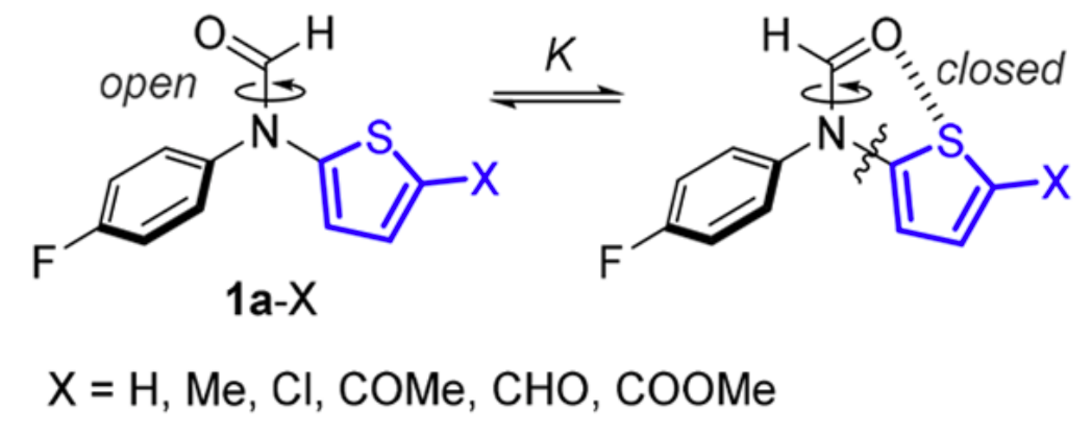
\includegraphics[width=0.6\linewidth]{Figures/cockroft-balances.pdf}
    \caption{``Molecular balances'' designed by \citeauthor[]{Pascoe2017} for the measurement of Ch-bond energies.\autocite{Pascoe2017}}
    \label{fig:cockroft-balances}
\end{figure}

DFT was used to further probe the dispersion contribution.
Free energies were calculated using functionals which both did, and did not include dispersion corrections, and the values compared to the experimental results.
The non-dispersion corrected B3LYP functional gave superior correlation with experiment than did either M06-2X and $\omega$B97-D, both of which include dispersion.
This provided additional evidence that, in the systems studied, the major contributor to the interaction is orbital overlap and charge transfer.

Although current evidence points towards these interactions being primarily orbital related, the electrostatic ``$\sigma$-hole'' terminology of Politzer and Murray has stuck, and the term is now used to encompass the whole gamut of X- Ch- Pn- and T-bonding interactions.

\section{Applications of Ch-Bonding}
Ch-bonding, and by extension, all $\sigma$-hole interactions can theoretically be applied to any formal Lewis acid-base system.
They are especially attractive as a hydro\emph{phobic} complement to H-bonding interactions, which are generally considered to be hydro\emph{philic}.
The following are brief summaries of existing applications in the literature.

\subsection{Materials}
The major applications of $\sigma$-hole interactions have so far been in the realm of crystal engineering.
Early work by \citeauthor{Corradi2000} showed that halogen bonding was able to outcompete H-bonding in the formation of supramolecular architectures.\autocite{Corradi2000}
A review by \citeauthor{Metrangolo2008} summarised the forms that are accessible using X-bonding to direct crystal growth.\autocite{Metrangolo2008}
1D, 2D, and 3D architectures are able to be generated using appropriate X-bond donors, and these show potential in the design of liquid crystals, organic semiconductors and paramagnetic materials (\cref{fig:iodotempo-chains})
A more recent review by the same group described applications in anion transport, and luminescent and photoresponsive crystals.\autocite{Priimagi2013}
The group of Stefan Matile has further explored anion transport, and has published a review comparing X-bonding with other hydrophobic interactions such as anion-$\pi$ and anion-macrodipole interactions (\cref{fig:matile-anion-binder}).\autocite{VargasJentzsch2013}

\begin{figure}
    \centering
    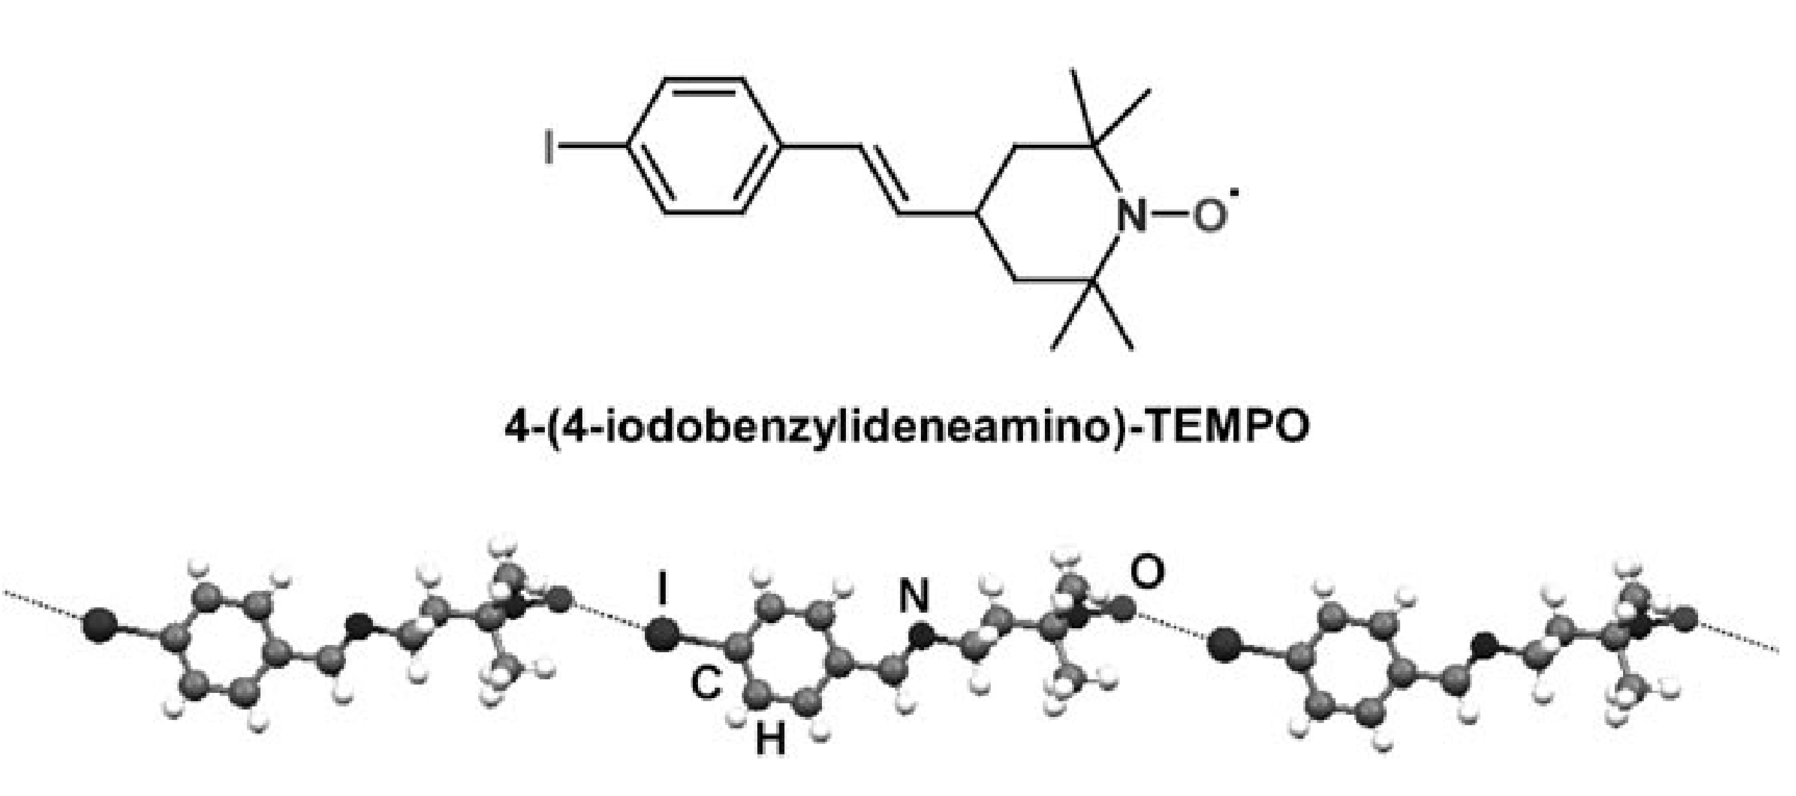
\includegraphics[width=0.6\linewidth]{Figures/iodotempo-chains.pdf}
    \caption{One-dimensional chains of 4-(4-iodobenzylidene)-TEMPO structured by X-bonds.\autocite{Metrangolo2008}}
    \label{fig:iodotempo-chains}
\end{figure}

\begin{figure}
    \centering
    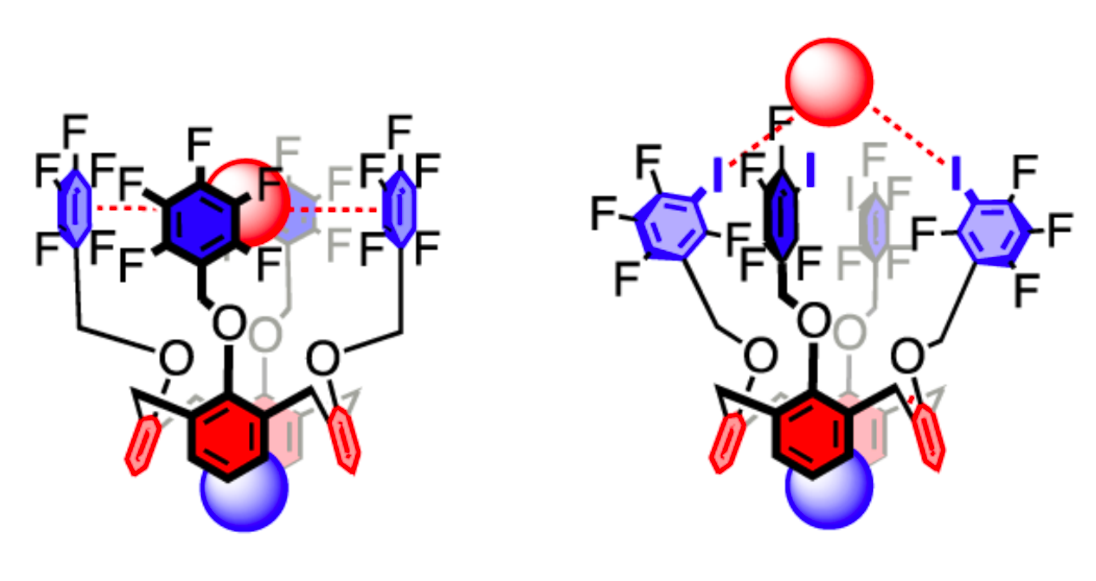
\includegraphics[width=0.4\linewidth]{Figures/matile-anion-binder.pdf}
    \caption{Anion binding through anion-$\pi$ interactions and X-bonding.\autocite{VargasJentzsch2013}}
    \label{fig:matile-anion-binder}
\end{figure}

Ch-bonding, too, has been investigated with respect to materials chemistry.
\citeauthor{Fanfrlik2014} demonstrated the importance of Ch-bonding on the crystal packing of thiaboranes.\autocite{Fanfrlik2014}
They found that the sulfur-based $\sigma$-hole was sufficiently strong to interact with the weakly basic $\pi$ electrons of a phenyl group, with contacts as short as 3.2\AA~being observed (\cref{fig:thiaborane-ch-bond}).

\begin{figure}
    \centering
    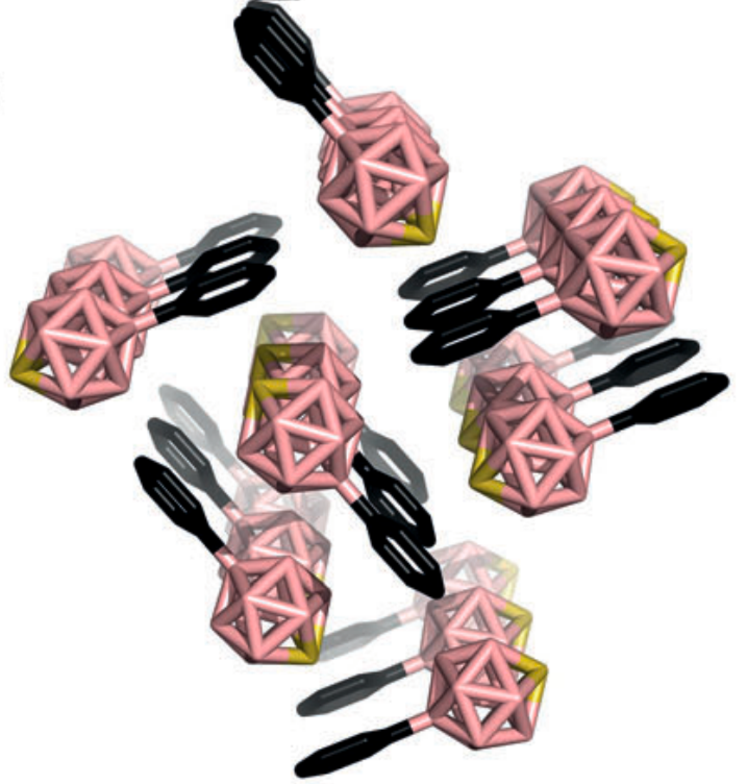
\includegraphics[width=0.3\linewidth]{Figures/thiaborane-ch-bond.pdf}
    \caption{Ch-bonding in thiaboranes.\autocite{Fanfrlik2014}}
    \label{fig:thiaborane-ch-bond}
\end{figure}

In 2016, \citeauthor{Ho2016} published their work into tellurium-based Ch-bonding.\autocite{Ho2016}
Their scaffolds are based on an iso-tellurazole N-oxide, which reversibly forms macrocyclic structures that persist in both gas and solution phase (\cref{fig:te-pd-macrocycle}).
The macrocycles were found to coordinate \ce{Pd2+}.
This is particularly interesting, as the tellurium atoms are simultaneously behaving as a Lewis acid and base.
The authors point out that such soft macrocycles are quite rare, and their work could facilitate further studies of transition metals in a soft coordination environment.
They went on to investigate benzo-fused derivatives of iso-tellurazoles, as well as selenium analogues, which crystallised to form macromolecular pores and voids.\autocite{Ho2017}

\begin{figure}
    \centering
    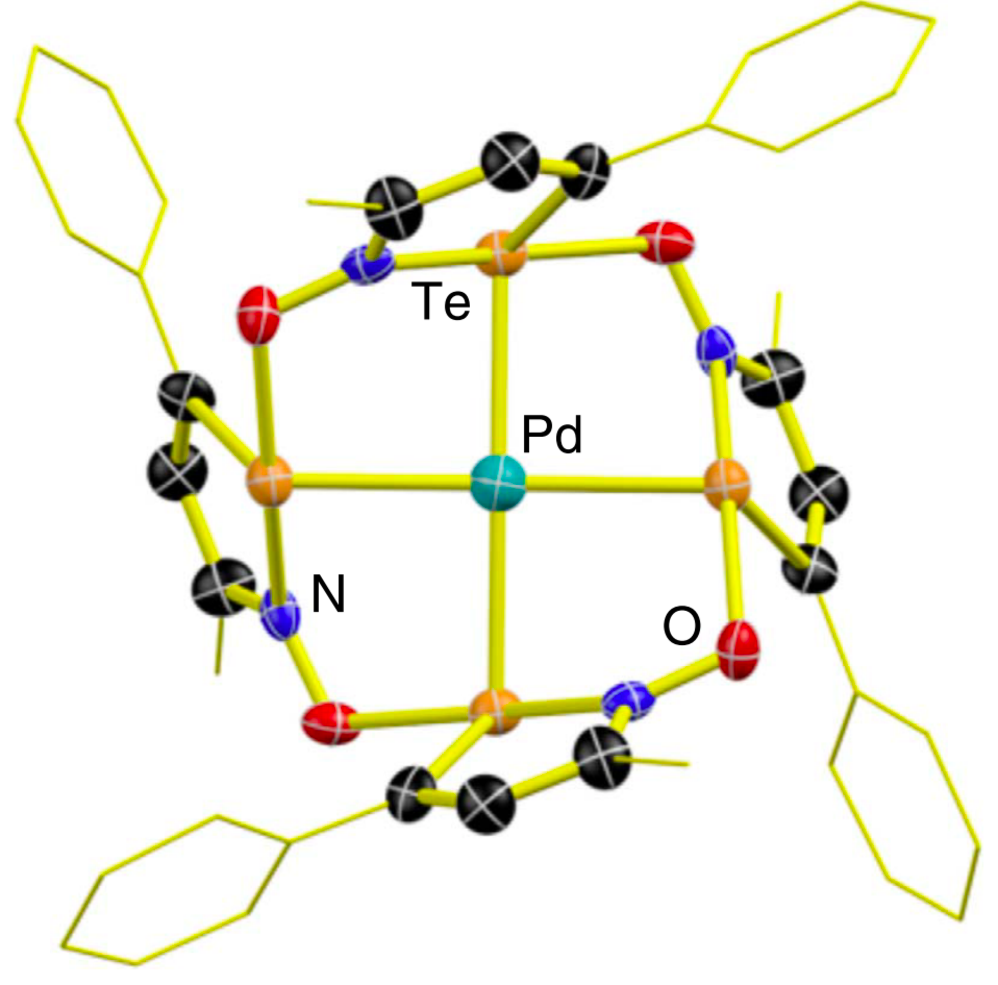
\includegraphics[width=0.4\linewidth]{Figures/te-pd-macrocycle.pdf}
    \caption{A tetrameric macrocycle held together by Ch-bonds.\autocite{Ho2016}}
    \label{fig:te-pd-macrocycle}
\end{figure}

The Taylor group has been active in the development of X- and Ch-bonding molecular sensors.
Early work demonstrated that X-bonding tridentate ligands (reminiscent of enterobactin) showed moderate selectivity for \ce{Cl-}.\autocite{Dimitrijevic2010}
They later developed bidentate Ch-bonding ligands which exhibited a tenfold increase in association constant with respect to chloride (\cref{fig:taylor-cl-binder}).\autocite{Garrett2015a,Garrett2016}

\begin{figure}
    \centering
    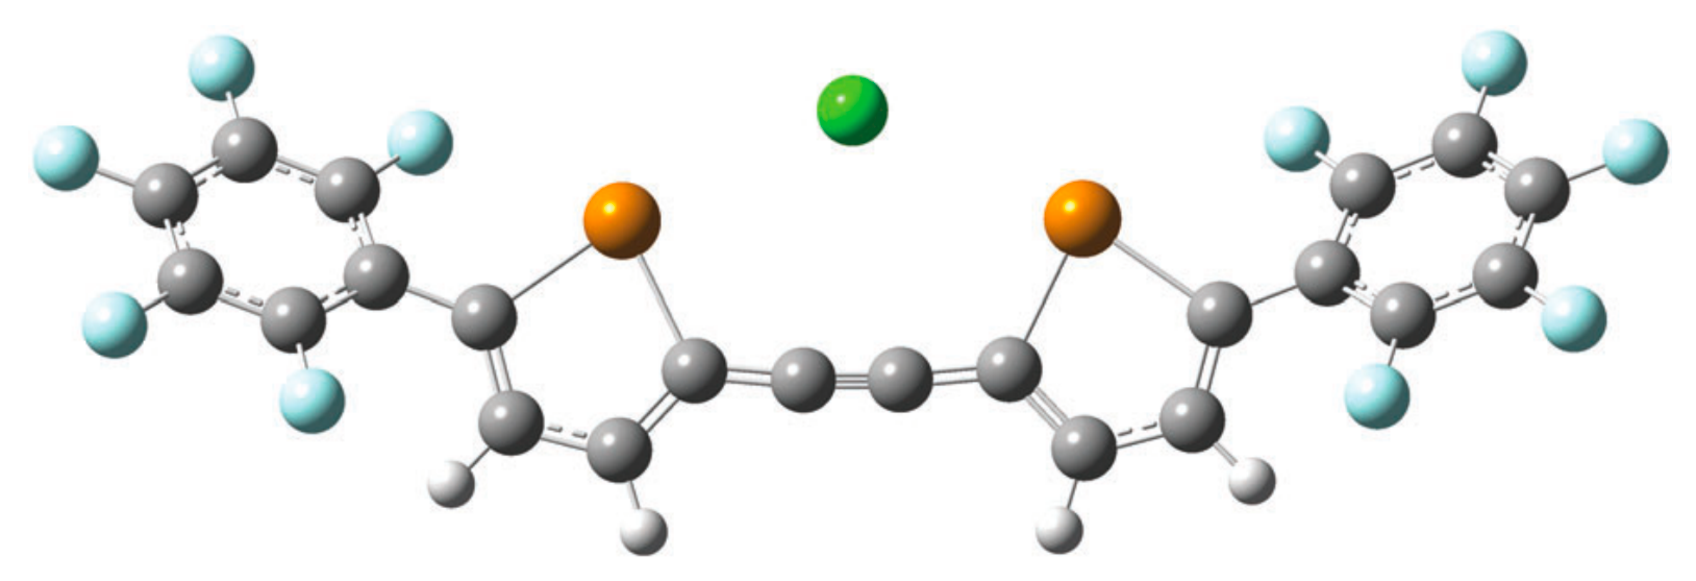
\includegraphics[width=0.6\linewidth]{Figures/taylor-cl-binder.pdf}
    \caption{A bidentate Ch-bonding anion binder.\autocite{Garrett2016}}
    \label{fig:taylor-cl-binder}
\end{figure}

Similar results have been achieved by the Beer group, who have developed X-bonding sensors for the perrhenate anion.\autocite{Cornes2017}
These sensors are based on functionalised cyclodextrins, and are even more sensitive than the corresponding H-bonding analogues.
The group has also use iodotriazole scaffolds to chelate anions.\autocite{Borissov2017}
Incorporation of a chial binapthol moiety was shown to differentiate between enantiomers of chiral anions.

The role of selenium-based Ch-bonding on the crystal structure and mechanism of the drug ebselen was demonstrated by Thomas et al.\autocite{Thomas2015}
Ch-bonding between the selenium atom and carbonyl oxygen directs the crystal packing of this compound, and leads to the formation of one-dimensional chains of molecules (\cref{fig:ebs-packing}).
Interestingly, the Lewis acidity of the $\sigma$-hole was invoked as an explanation of the antioxidant properties of the drug.

\begin{figure}
    \centering
    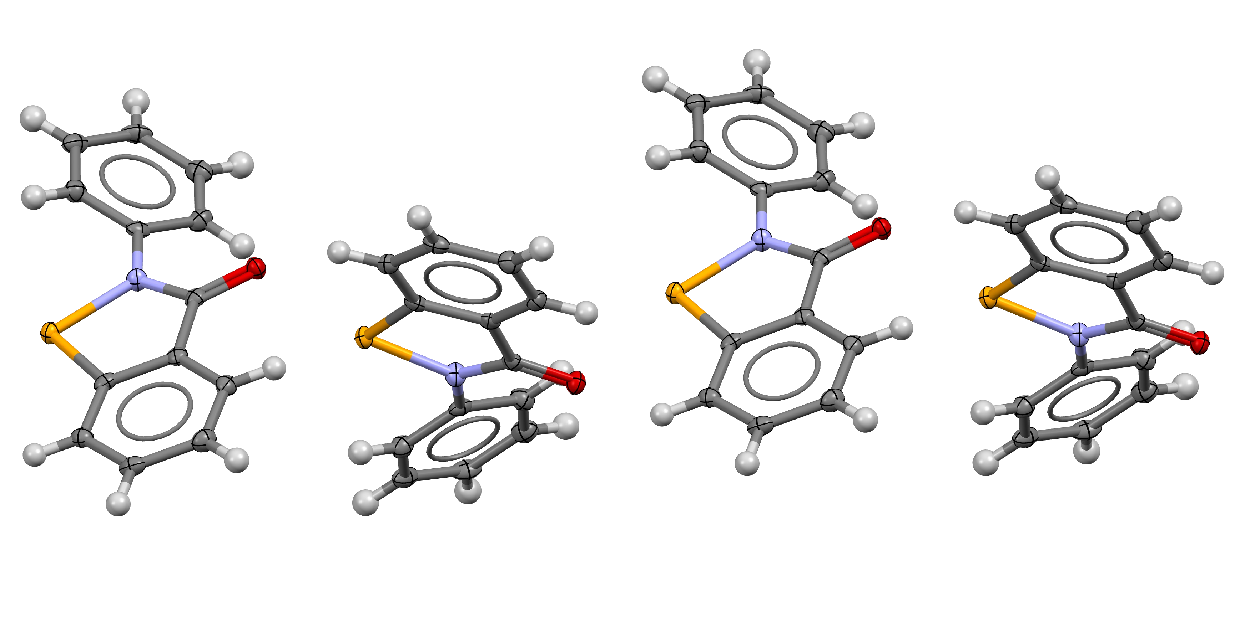
\includegraphics[width=0.7\linewidth]{Figures/ebs-packing.pdf}
    \caption{One dimensional chais formed in the crystal packing of ebselen.}
    \label{fig:ebs-packing}
\end{figure}

\subsection{Catalysis and bond activation}
In 2008, halogen bonding was first applied to a Hantzsch ester reduction of a quinoline derivative.\autocite{Bruckmann2008}
This reaction is well characterised and understood, and has been catalyzed with a variety of Br\o nsted and Lewis acids.
The X-bond donors chosen were perfluoroiodoalkanes, and high conversions were achieved with modest catalyst loadings of 10\%.

In 2011, a modified Ritter reaction was devised wherein benzhydryl bromide was activated by a dicationic imidazolium-based X-bond donor to give the carbocation intermediate, which was then captured by acetonitrile and then hydrolysed to afford the amide product.\autocite{Walter2011}
This pioneering work was limited by the necessity of stoichiometric amounts of the X-bond donor, as it is consumed in the course of the reaction.

A similar alkylation of 1-chloroisochroman was achieved by the same group using a neutral perfluoroiodoarene X-bond donor in catalytic quantities.\autocite{Kniep2013}
The proposed mechanism is similar to the thiourea-catalysed reaction of \citeauthor{Reisman2008}\autocite{Reisman2008}, which has shown promise in asymmetric induction.
The authors noted issues with solubility of the perfluoroiodoarene catalysts, which is expected of such highly fluorinated compounds.

The reduction of quinoline was sucessfully catalysed by a dithiophene system by \citeauthor{Benz2017} in 2017\autocite{Benz2017}, and then again by the same group with a benzodiselenazole (\cref{fig:quinoline-redn}).\autocite{Benz2017a}
With the increased selectivity and strength of the Se-based Ch-bonding catalyst compared to the X-bonding perfluoroiodoalkane, the authors were able to reduce the catalyst loading to 1\%.

\begin{figure}
    \centering
    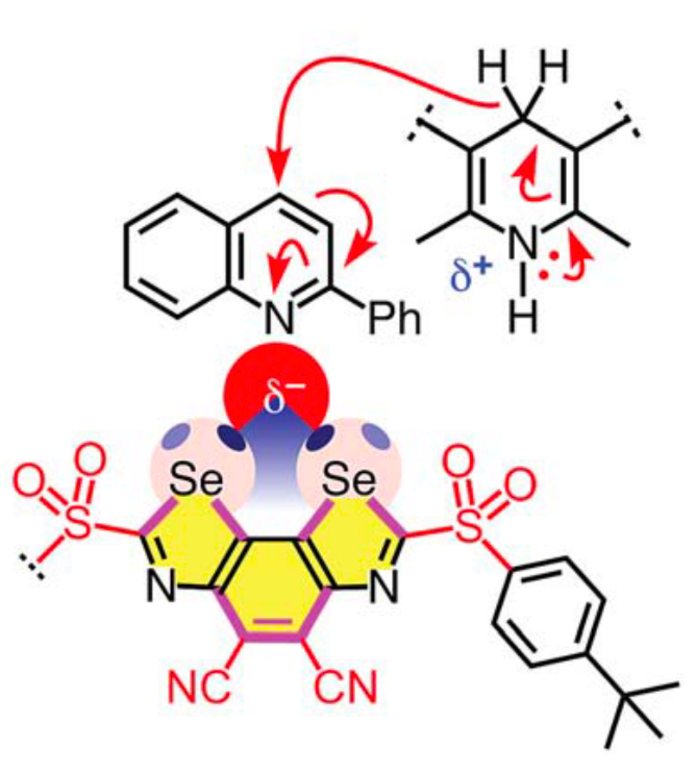
\includegraphics[width=0.4\linewidth]{Figures/quinoline-redn.pdf}
    \caption{Proposed mechanism for the catalytic reduction of quinoline by a Ch-bonding catalyst.\autocite{Benz2017}}
    \label{fig:quinoline-redn}
\end{figure}

\citeauthor{Wonner2017} developed a selenated bisbenzimidazolium Ch-bonding catalyst for the alkylation of 1-chloroisochroman, and solvolysis of benzyhydryl bromide.\autocite{Wonner2017,Wonner2017a}
Although the best results were observed with the dicationic catalysts, conversion was also achieved with a neutral bisbenzimidazole catalyst, providing further evidence that the catalytic Lewis-acid site is indeed the $\sigma$-hole.
For a given row in the periodic table (i.e. comparing a Se-based donor to a Br-based donor), Ch-bonding appeared to give superior results to X-bonding, as measured by \% yield.

An unusal manifestation of X-bonding is in the self-disproportionation of enantiomers, as reported by \citeauthor{Soloshonok2017}.\autocite{Soloshonok2017}
They observed spontaneous enrichment of one enantiomer of mebroqualone (\cref{fig:mebroqualone}) upon chromatography using an achiral solid phase, which they attributed to the formation of diasteromeric X-bonded oligomers.
This phenomenon has been observed in compounds capable of interacting through H-bonding or strong dipole-dipole interactions.\autocite{Cundy1983}

\begin{figure}
    \centering
    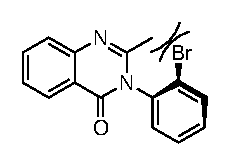
\includegraphics[scale=0.8]{Figures/mebroqualone.eps}
    \caption[The structure of mebroqualone.]{The structure of mebroqualone. Rotation is hindered about the biaryl bond, allowing the isolation of two atropisomers.}
    \label{fig:mebroqualone}
\end{figure}

\subsection{Biological systems}

\subsubsection{Proteins}
While we usually think of the tertiary structure of proteins as being dominated by H-bonding and hydrophobic effects, there is increasing evidence that Ch-bonding plays an important role as well.
This is not unexpected, as sulfur, a component of both cysteine and methionine, is known to form Ch-bonds in small molecules.
In the early days of Ch-bonding interactions (2001, before the name had come into common use) \citeauthor{Iwaoka2001} published an analysis of 604 protein structures in the Protein Data Bank (PDB).\autocite{Iwaoka2001}

A remarkable number of close contacts (sum of Van der Waals radii plus 0.5\AA) between sulfur and Lewis basic (X) atoms were identified in the structures, with 33\% of cysteine residues and 22\% of methionine residues showing a close contact.
Furthermore, the geometric parameters of these contacts were studied, with more than half of all contacts having a S--S--X (X=O,N) of 150--180\degree.
The observed contacts were ascribed to a $\pi$(C=O)$\rightarrow \sigma^{\star}$(S--S) interaction, in contrast to the $n(X) \rightarrow \sigma^{\star}$(S-X) interaction which dominates in small molecules.
Also contrary to the case of small molecules, the authors suggested that the orbital component of the interaction is small, though important for establishing the directionality of the interaction.
Dispersion appears to be the major stabilising force, as optimization using a non-dispersion corrected level of theory gave unrealistically large distances.

The differences between Ch-bonding in proteins and small molecules is likely due to variation in orbital energies in the functional groups which are found in each class.
While small molecule Ch-bond donors are characterised by easily accessible, low energy $\sigma^{\star}$(Ch--X) orbitals, these are simply not found in proteins.
Instead, donors are characterised by $\sigma^{\star}$(S--S) or $\sigma^{\star}$(S--C) orbitals, which are much higher in energy and less accessible to acceptors.
Ch-bond acceptors, too, are markedly different between small molecules and proteins.
In general, the HOMO of a system (the most Lewis basic site) is dominated by lone pairs.
This is observed in most small molecules, as they form Ch-bonds through these lone pairs.
However, the amide bond, which is ubiquitous in proteins, shows an unusual inversion in orbital energies.
The $\pi$(C=O) orbital is elevated with respect to the lone pair according to MP2 calculations, making it the more basic site.
Structural data supports this assertion, as the Ch-bond donor usually approaches the top of the C=O bond in proteins, rather than the usual approach towards the oxygen lone pair (\cref{fig:amide-diselenide-ch-bond}).\autocite{Iwaoka2012}

\begin{figure}
    \centering
    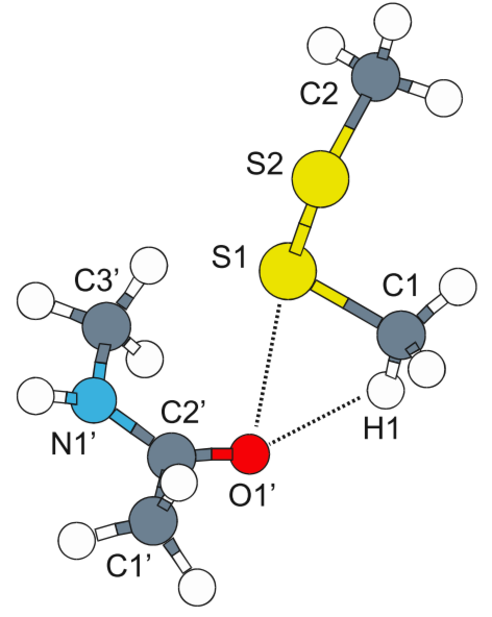
\includegraphics[width=0.4\linewidth]{Figures/amide-diselenide-ch-bond.pdf}
    \caption{Directional preference for Ch-bonded interactions in proteins.}
    \label{fig:amide-diselenide-ch-bond}
\end{figure}

It is worth noting that selenium is also found in proteins as selenocysteine and selenomethionine.
This would be expected to be an even stronger Ch-bond donor.
However, selenoproteins are relatively few in number, precluding such extensive statistical analysis.\autocite{Iwaoka2015}
They are only mentioned here for the sake of completeness.

Intramolecular interactions are just one instance of Ch-bonding in biological systems.
Proteins often interact with ligands or substrates through H-bonds, so it is reasonable to propose that Ch-bonding could be applied in this field as well.
Indeed, a protein-ligand Ch- and X-bonding interaction was used to target the gatekeeper methionine (MET146) residue of c-Jun N-terminal kinase 3 (JNK3) in a model study by \citeauthor{Lange2015}.\autocite{Lange2015}
In this work, a protein$\rightarrow$ligand Ch-bond was used to stabilise the interaction.
Inhibition of a cysteine protease using a variety of sulfur-containing heterocyclic ligands was also investigated.\autocite{Giroud2017}
These ligands formed ligand$\rightarrow$protein Ch-bonds, complementary to the the work by Lange.
Non-conventional protein-ligand interactions are summarised in a comprehensive review by Beno et al.\autocite{Beno2015}

\subsubsection{Nucleic acids}
Nucleic acids represent another application of Ch-bonding in biology.
In addition to their crucial role in the storage of genetic information, they have also been investigated as a structural material in nanotechnology.
The ubiquity of H-bonds in nucleic acid complexes suggests that $\sigma$-hole interactions may also be used to direct formation of these complexes.
X-bonding was indeed able to be used to direct formation of a Holliday junction between two DNA strands (\cref{fig:holliday-junction}).\autocite{Voth2007}
Holliday junctions are branched nucleic acid structures that appear in many biological processes includin recombination and double-strand break repair.
They are also useful as building blocks for DNA nanotechnology, where their self assembly and predictable gemoetry are exploited.
The authors estimated that the X-bonding interaction (mediated through a bromo-substituent) was 2--5 kcal/mol stronger than the corresponding H-bond.
A 2017 review identified a further 21 X-bonded nucleic acid structures.\autocite{Kolar2017}
X-bonding was in fact able to partially replace inter-strand H-bonding interaction in a DNA oligomer.\autocite{Parker2012}

\begin{figure}
    \centering
    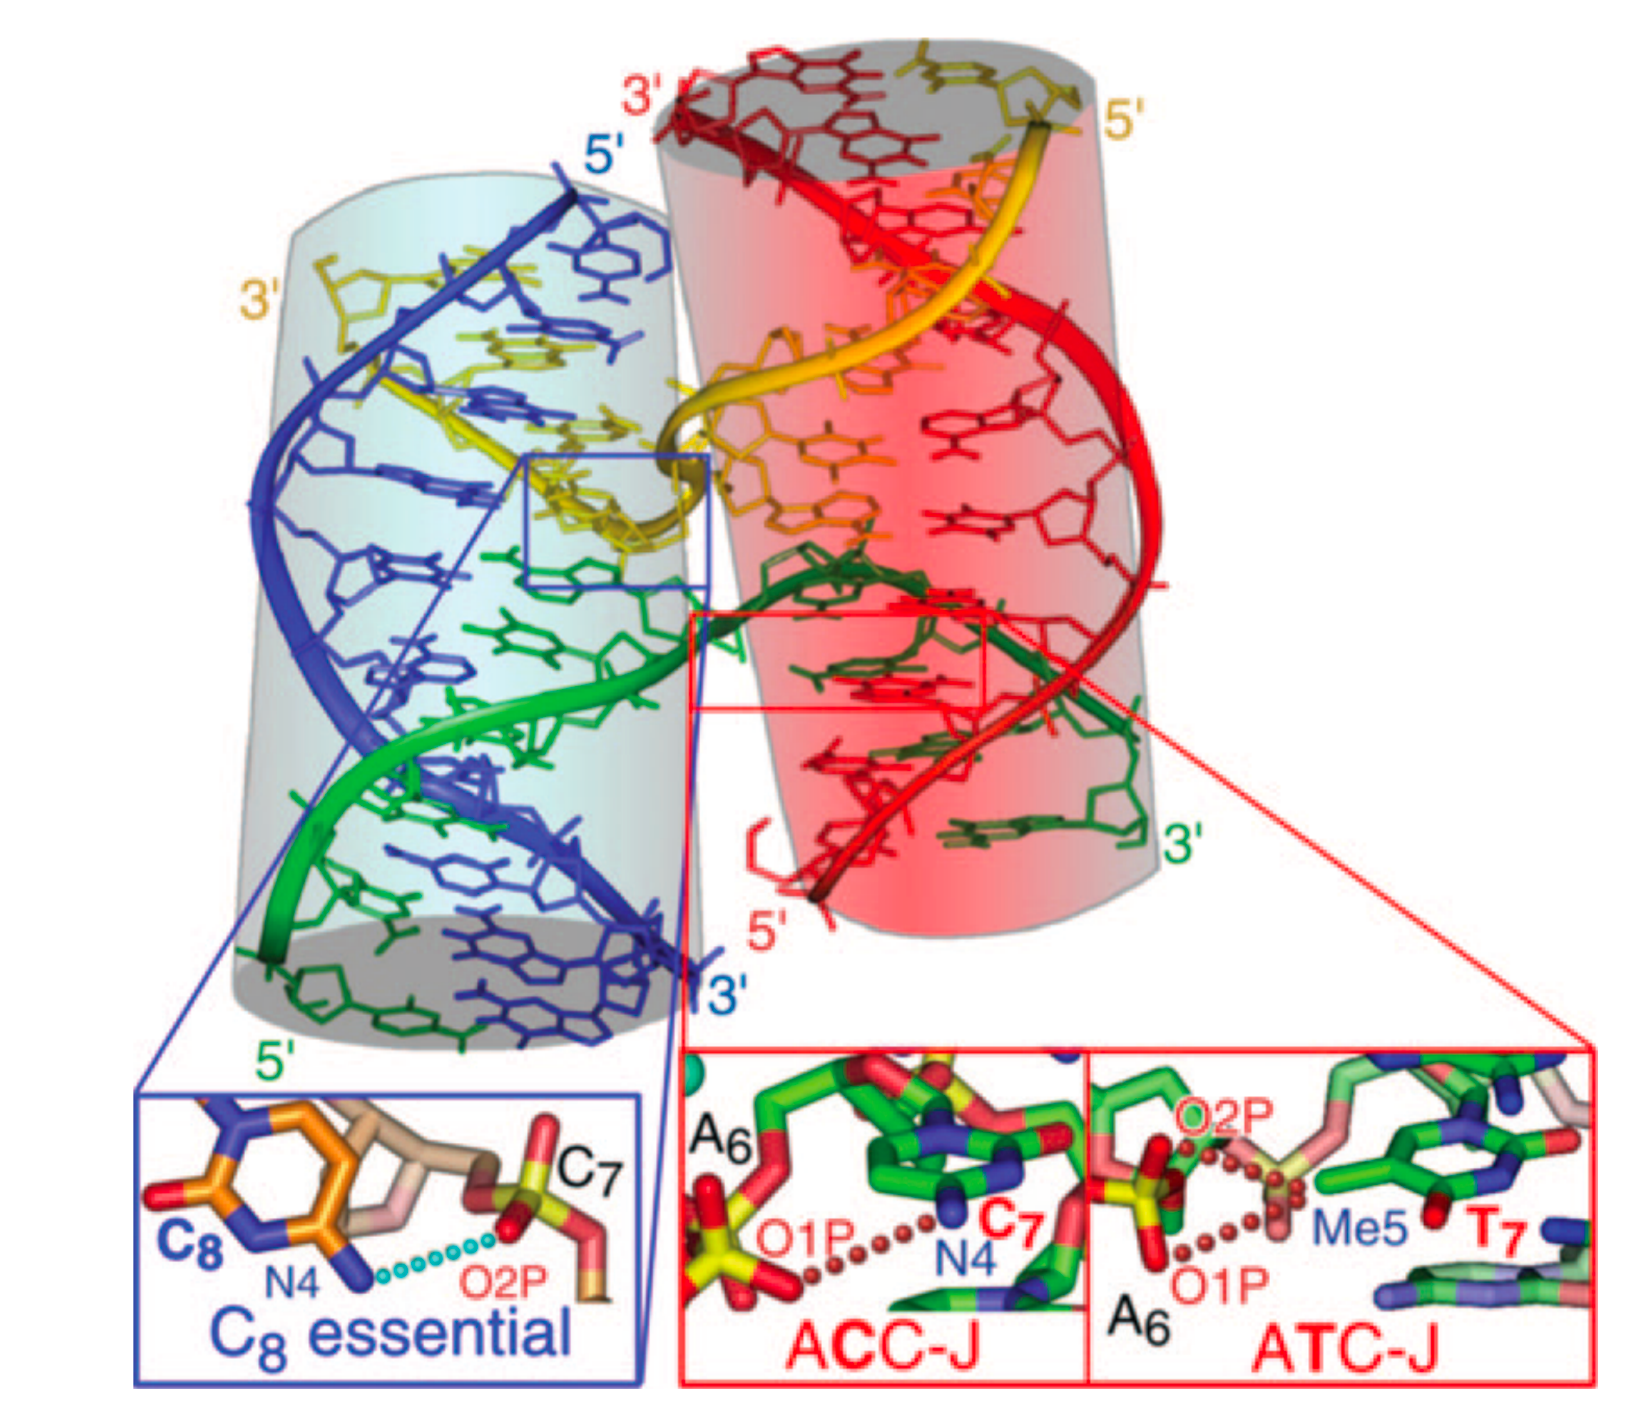
\includegraphics[width=0.4\linewidth]{Figures/holliday-junction.pdf}
    \caption{Holliday junction formed by X-bonding.\autocite{Voth2007}}
    \label{fig:holliday-junction}
\end{figure}

Ch-bonding, too, has been investigated in the context of nucleic acids.
\Citeauthor{Sharma2020} recently invesigated the possibility of forming Ch-bonded analogues of the canonical A:T/G:C base pairs in order to expand the genetic alphabet.\autocite{Sharma2020}
A G\textsubscript{\ce{SeF}}:C dimer was found to be more stable than the canonical G:C pair, where the \ce{SeF} subscript indicates that one of the H-bond donors on the guanine was replaced by a selenenyl fluoride.
\Citeauthor[]{Farrell2018} showed that introducing heavy chalcogens into nucleobases has profound impacts on their phototochemistry, with implications for their use in photodynamic therapy.\autocite{Farrell2018}
The photophysics of selenonucleobases has been further explored, showing that they are uniquely photostable while efficiently populating and depopulating their excited states.\autocite{Mai2019,Peng2020,Fang2019,Uleany2020}
While none of these investigations specifically mentioned Ch-bonding, it is highly likely that it would come into play, which may provide a means of directing the activity of these photosensitisers.
Selenium has also been incorporated into nucleobases as a H-bond acceptor, in which it was shown that selenonucleobases can effectively discriminate against the formation of a so-called ``wobble'' base pair (U:G as opposed to U:A in RNA, or T:G/T:A in DNA).\autocite{Hassan2010,Sun2012}
Another advantage of selenonucleobase incorporation is the ability to use the heavy selenium atom for MAD/SAD phasing of macromolecular crystal structures.\autocite{Salon2007}
This was also the motivation for a \citeyear{Conlon2019} study in which the selenium was incorporated into the phosphate backbone.\autocite{Conlon2019}
A major advantage of this approach is that the bulk of the selenium atom does not need to be accomodated in the interior of the double helix, so structural distortions are minimised.
To date, there have not been any drugs which target nucleic acids through Ch-bonding, which is an area we explore in \cref{ch:dna-binder}.

\section{Experimental methods}
As mentioned above, X- and Ch-bonded interactions were originally identified crystallographically, with additional spectroscopic evidence being present.
These pioneering methods have not changed a great deal, and x-ray crystallography is still the most powerful tool we have to study these interactions.
We also use a number of spectroscopic techniques to probe the nature of Ch-bonding.
Some of the methods used in this thesis are explained below.

\subsection{Computational methods}

\subsubsection{Energy Decomposition Analysis}

\subsubsection{Natural Bond Orbital theory}

\subsubsection{Quantum Theory of Atoms In Molecules}

\subsection{X-ray crystallography}
Single crystal x-ray crystallography is the main experimental technique used in this work.
It allows unambiguous determination of the structure of compounds (including stereochemistry), and  extremely accurate measurement of geometric parameters such as bond lengths.
Practically speaking, a structure is determined by mounting a single crystal of a compound on a goniometer which can rotate the crystal through any orientation, then observing the position and intensity of diffracted x-ray beams.
Rotating the crystal allows different diffraction spots to be observed, and a more complete dataset to be collected.
The position of the diffraction spots provides information about the size and shape of the unit cell, and the intensities provide information about the internal structure i.e. the locations of the atoms in the unit cell.
A full discussion of the mathematics of diffraction is outside the scope of this thesis, but the interested reader is referred to \citetitle{Stout1989} by \citeauthor{Stout1989}.\autocite{Stout1989}

\subsubsection{Charge density refinement}
Fundamental to the technique of x-ray structure determination is the process of refinement, by which parameters of the model (typically the molecular geometry) are optimised to reproduce the observed intensity data as well as possible.
Mathematically, this is performed as a least-squares optimisation, where the function
\begin{equation}
    \sum^{m}_{r=1} w_{r} \left(f_{\mathrm{obs}, r} - f_{\mathrm{calc}, r} \right) ^{2}
\end{equation}
is minimised, where $f_{\mathrm{obs}, r}$ corresponds to the observed intensity, and $f_{\mathrm{calc}, r}$ corresponds to the intensity calculated from the model by Fourier transform.
$w_{r}$ is a weighting function used to reflect the confidence in any given observed data point.

Assuming the measured intensities are free of any error,\footnote{This is practically never the case, but careful measurement and modern corrections can approach this limit.} this function could theoretically be minimised to zero i.e. the model is a complete and true representation of the crystal.
The question then becomes, how do we determine $f_{\mathrm{calc}, r}$ from our model?
To answer this, we must consider what our model actually \emph{is}.

The simplest refinement model consists of atomic coordinates for each atom, plus an overall scale factor (for now we will neglect the anisotropic displacement parameters and chemical occupancies).
However, in order to calculate $f_{\mathrm{calc}, r}$ by Fourier transform, we must introduce some description of what the atoms which we are locating ``look like''.
This forms a hidden, but still crucially important, part of the model.
Typically, atoms are described in reciprocal space as spherically symmetric functions whose contribution to $f_{\mathrm{calc}, r}$ is only dependent on $(\sin\theta)/\lambda$ (\cref{fig:scatterf}).
This is a consequence of the fact that x-rays are scattered by the \emph{electron cloud} of the atom.\footnote{X-rays have much less energy than the mass-energy of subatomic particles, and so are scattered in the low energy limit of Compton scattering, known as Thompson scattering.
The scattering power of a particle is inversely proportional to the square of its mass, so the massive nuclei contribute negligibly to scattering compared to electrons.}
At $(\sin\theta)/\lambda = 0$ the scattering factor is equal to the number of electrons in the atom.
However, the finite size of the electron cloud causes destructive interference and attenuation of the scattering factor as $(\sin\theta)/\lambda$ increases, as x-rays scattered from one side of the electron cloud will be out of phase with those scattered from the other side.
Contrast this with neutron diffraction, where the neutrons are scattered predominantly by the point-like nucleus, affording a flat scattering function in reciprocal space.
There is almost no destructive interference, and thus neutron crystallography is characterised by an abundance of strong high angle data.
The scattering factor functions for all elements of the periodic table (and many ions) have been calculated based on theoretical electron densities from Hartree-Fock wavefunctions, and the results are available in the International Tables.\autocite{IntTabCIntensityofdiffractedintensities}
These functions are mercifully incorporated in crystallographic refinement software, shielding them from the user.

\begin{figure}
    \centering
    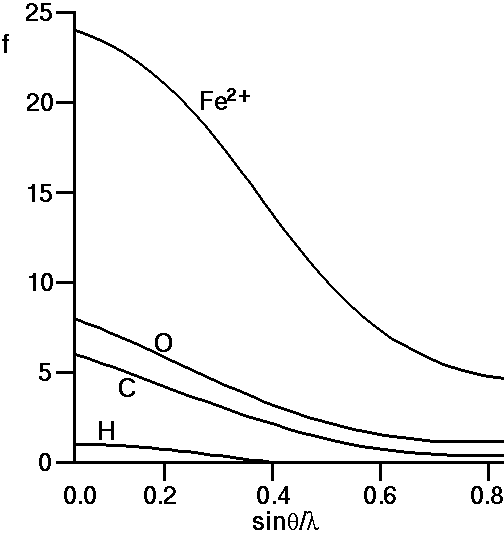
\includegraphics[width=0.5\linewidth]{Figures/scatterf.png}
    \caption{Scattering factors for some atoms as a function of $(\sin\theta)/\lambda$.}
    \label{fig:scatterf}
\end{figure}

From the above discussion, one major shortcoming of this approach should be clear.
Namely, that the electron density of bonded atoms is \emph{not} spherically symmetric.
Perturbations such as bonding electron density, lone pairs, and indeed $\sigma$-holes can, and do, affect the observed scattering factors of atoms, which are not taken into account in typical refinement software.
An extreme case of this, and one that is familiar to any crystallographer, is that of the hydrogen atom.
As the lightest element with only one electron, perturbations due to bonding have an enormous effect, such that the typical \ce{C-H} bond length is underestimated by some 0.13~\AA.\autocite{Cooper2010}
A subtler but more interesting manifestation of this was identified in 1968 by \citeauthor{Coppens1968EvidenceEffects}.\autocite{Coppens1968EvidenceEffects}
X-ray and neutron structures were determined for a crystal of 1,3,5-triazine, and inspection of the difference (a so-called $\mathrm{X}-\mathrm{N}$ map) revealed unusual systematic variations in the anisotropic displacement parameters.
The nitrogen atoms were deformed radially to the ring, while the carbon atoms were deformed tangentially (\cref{fig:x-n-coppens}).
This is chemically intuitive, as we would expect the lone pairs of the nitrogens to extend radially, while the $\pi$-electrons of the carbon atoms would form a ring.
The fact that these deformations were incorporated into the anisotropic displacement parameters in the x-ray structure highlights a deficiency of the typical method of refinement.

\begin{figure}
    \centering
    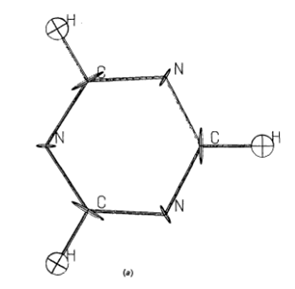
\includegraphics[width=0.5\linewidth]{Figures/x-n-coppens.png}
    \caption[Structure of 1,3,5-triazine.]{$\mathrm{X}-\mathrm{N}$ map of 1,3,5-triazine, reproduced from \citeauthor{Coppens1968EvidenceEffects}.\autocite{Coppens1968EvidenceEffects}}
    \label{fig:x-n-coppens}
\end{figure}

Evidence for aspherical atoms can even be traced back to seminal studies performed by \citeauthor{Bragg1920}, in which the famous 222 reflection of a diamond crystal was observed.
The 222 reflection is a systematic extinction of the $Fd\bar{3}m$ space group to which diamond belongs, but its absence is based on the assumption of spherical atoms.
In diamond, the carbon atoms are actually tetrahedral in form due to the bonding electron density, which lowers the space group symmetry and causes the 222 reflection to be present, though very weak.\autocite{Bragg1920}
Though cutting edge for the time, Bragg's experiment was rather primitive, and multiple scattering likely contributed some intensity to the observed 222 reflection.
The observation was nonetheless correct, and the tetrahedral nature of the carbon atoms in diamond has subsequently been proven time and time again.

Although such perturbations generally only manifest in very high quality structures (aspherical atoms are typically the least of a crystallographer's worries), a number of methods have been proposed to improve refinements, and indeed gain further chemical knowledge from the experimentally determined aspheical electron density.
A simple approach is the use of tabulated aspherical scattering factors for atoms of distinct chemical types.
An example of this is the ELMAM2 database, developed by Jelsch and coworkers.\autocite{Domagaa2012}
The ELMAM2 database consists of experimentally derived scattering factors for all common atom types, with a focus on those found in amino acids and peptides.
A refinement using this database would begin by assigning a type to each atom, which can be done relatively easily using bonding geometries from a more primitive refinement.
This can afford substantial improvement in refinement statistics by providing a more accurate model, at a very modest computational cost.
The obvious drawback of this approach is that the scattering factors must already be tabulated, and the enormous diversity beyond the biochemically important C, H, N, and O precludes the assembly of a truly comprehensive database.
Furthermore, as the scattering factors are pre-tabulated, there is little chemical information that can be extracted from the model beyond somewhat improved precision in geometric parameters.

An improved approach is to compute scattering factors on a case-by-case basis.
This is the rationale behind Hirshfeld Atom Refinement (HARt), first developed by \citeauthor{Jayatilaka2008}.\autocite{Jayatilaka2008}
HARt is an iterative procedure in which the atomic coordinates from a spherical atom refinement (perhaps after correcting \ce{C-H} bond distances) are used to variationally calculate a wavefunction, from which is calculated an electron density and thus scattering factors.
These new scattering factors improve the model after refinement, from which is calculated a \emph{new} wavefunction, and so on until the cycles of least squares refinement and wavefunction calculations converge.
Clearly this repeated calculation of a wavefunction is computationally expensive, with even relatively simple molecules taking minutes.
Fortunately, however, even very inexpensive levels of theory tend to generate sensible densities for the ground state.
An advantage over the database approach is that one can capture unusual effects in the electron density (such as various non-bonding interaction), provided that they are correctly modelled by the underlying quantum chemistry theory used to generate the wavefunction.
However this raises a philosphical question: what exactly we are hoping to get out of this procedure?
It can certainly provide improved refinement statistics, including anisotropic refinement of hydrogens in agreement with neutron data, but if we are seeking chemical information about the system, we might as well simply use a gas-phase optimised wavefunction and dispense with the crystallography.

Related to this is the field of quantum crystallography, which differs somewhat in motivation, if not in methodology.
Quantum crystallography is concerned with extracting a wavefunction from diffraction data, rather than using a wavefunction to improve a crystallographic model.
Clearly there is significant overlap.
One method takes inspiration from perturbation theory, where, as in MP2, the Hartree-Fock wavefunction is taken as the zeroth order approximation.
The diffraction data is then used to construct a perturbative term, which introduces a degree of correlation to the wavefunction, bringing it closer to the truth (at least within the Born-Oppenheimer approximation).\autocite{Weiss1962}
Even with the power of modern computers, this is not an easy task, and quantum crystallography remains an active and exciting area of research.
It is also worth mentioning the x-ray constrained wavefunction method developed by \citeauthor{Grimwood2003}.\autocite{Grimwood2003}
This is simply a Hartree-Fock wavefunction calculations that is constrained via a Lagrangian multiplier to reproduce the observed intensities in the experimental data, assuming there are no crystallographic artifacts in the data such as disorder or twinning.
That is to say, the crystal is simply comprised of infinitely repeating symmetry related molecular units.
The x-ray constrained wavefunction can be used to calculate a density, which can be used in a HARt-like procedure, which has been named x-ray wavefunction refinement (XWR).\autocite{Woinska2017}
Both quantum chemistry and crystallographic refinement codes have been implemented in the software package TONTO.\autocite{Jayatilaka2003}

Perhaps the most powerful approach for experimental crystallographers is that of multipole refinement using the formalism developed by Hansen and Coppens.\autocite{Hansen1978}
While superficially similar to quantum crystallographic approaches, no chemical restraint\footnote{This is not strictly true, as electroneutrality is routinely imposed as a constraint on multipole models.} is placed on the resulting electron density, allowing for the modelling of phenomena which are not described by \emph{ab inito} calculations.
The electron density is expanded in a series of atom-centered spherical harmonic basis functions, the local coordinate systems of which are often chosen to align with chemical features.
Each basis function requires two parameters for the occupancy and expansion, in addition to the position and anisotropic displacement parameters for each atom.
We therefore require a large number of observations to ensure the system is overdetermined, and can be treated in a least-squares manner.
Furthermore, the ADPs and dipolar basis terms are highly correlated, leading to an unstable solution if refined simultaneously (\cref{fig:adp-dipole}).

\begin{figure}
    \centering
    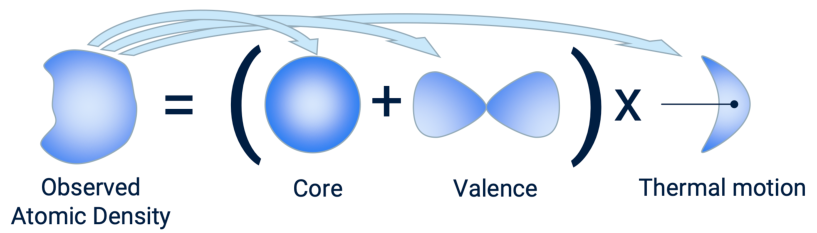
\includegraphics[width=0.6\linewidth]{Figures/valencevsthermaled.pdf}
    \caption[Correlation of thermal and dipolar functions.]{Thermal motion (described by anisotropic displacement parameters) and dipolar basis terms are highly correlated.}
    \label{fig:adp-dipole}
\end{figure}

For this reason, it is critical to establish accurate atomic positions and ADPs before refining the multipole parameters and charge density.
Traditionally this was done using neutron data which, as mentioned above, is insensitive to electron density perturbations as neutrons are scattered almost exclusively by the nucleus.
Unfortunately neutron sources are notoriously expensive and low-flux, requiring extremely large crystals which introduces further errors due to extinction.
With the advent of modern x-ray diffractometer technology, we can luckily determine atomic coordinates and ADPs using x-ray data alone.
This is done using high angle reflections, which are dominated by core scattering and thus contain little data from the diffuse bonding electron density.
Core electron density is almost perfectly spherical, allowing ADPs to be correctly refined from this data.
With accurate atomic coordinates and ADPs in hand, hydrogen atoms can be located in the low angle data, and then the multipole parameters refined to convergence.
Multipole refinement can benefit enormously from an initial database model, particularly for hydrogen atoms, so it is no surprise that the techniques are often used sequentially.\autocite{Guillot2001,Volkov2006}
The resulting electron density can be used to characterise molecules and predict reactivity, particularly when interpreted within the powerful Quantum Theory of Atoms In Molecules frameork of Bader.\autocite{Bader1991}
The obvious attraction of this method is that it is almost entirely experimental.
However, the atom centered multipole functions and their resulting sum, while superficially resembling a wavefunction, is not antisymmetric and is therefore in violation of the Pauli exclusion principle.
It therefore cannot be used to determine \emph{all} properties of a system.

To summarise, electron density can be measured in a crystal by x-ray diffraction, and various models used to fit it.
The ``gold standard'' would be the derivation of a wavefunction, but at present this has not been done without the introduction of chemical constraints.
In practise, the most accurate and most informative fitting of electron density to diffraction data is done with a series of atom-centered spherical harmonic functions (the Hansen-Coppens formalism).
The resulting electron density can be used in QTAIM analysis, or used to construct electrostatic potential maps, which can guide chemists in their understanding of molecules in crystals.

\subsection{Nuclear Magnetic Resonance}
Nuclear magnetic resonance spectroscopy (NMR) is an essential tool for all organic chemists, as it is able to give relatively detailed structural information quickly and cheaply.
It is based on the magnetic moment of certain nuclei, which are usually randomly oriented but spontaneously align in the presence of a strong magnetic field.

\subsubsection{Solid State NMR}
The chemical shift of a nucleus is not a simple scalar quantity, as solution phase NMR experiments might suggest.
The shielding, and hence the effective magnetic field felt by the nucleus depends on the electronic environment around the nucleus, which is decidedly \emph{an}isotropic, therefore incapable of being expressed as a scalar.
Depending on the orientation of the electron cloud (and other shielding/deshielding influences) around the nucleus with respect to the magnetic field, different chemical shifts will be observed for the same nucleus.
This phenomenon is the chemical shift anisotropy of a nucleus, and it is described mathematically by a second rank tensor, which is geometrically depicted as an ellipsoid.

In a solution phase NMR experiment, rapid and random tumbling of the molecules averages out the anisotropy of each signal, affording a sharp peak at the isotropic chemical shift.
This can be simulated to some degree by magic angle spinning in solids experiments, but it is often the case that the chemical shift anisotropy is more interesting that the isotropic shift, so a solid phase NMR experiment is the only way to examine it.

The shape of the chemical shift tensor can provide insight into the electronic environment of a nucleus, with large shielding components often being aligned with electronic features such as bonds or lone pairs.
It is often convenient to define a principal axis system (PAS) for the tensor, consisting of two components which describe the longest and shortest axes of the ellipsoid, and the axis perpendicular to both.
The PAS of the chemical shielding tensor is denoted by the lowercase $x$, $y$ and $z$, and the components of the tensor which are aligned with these axes are labelled $\sigma_{xx}$, $\sigma_{yy}$ and $\sigma_{zz}$.
The laboratory reference frame is denoted by the uppercase $X$, $Y$ and $Z$, with the magnetic field $B_0$ being aligned with the $Z$ axis.
A common method for transforming one coordinate system to another is through the use of Euler angles $\alpha$, $\beta$ and $\gamma$, which define sequential right-handed rotations about the axes of the rotating frame.
As the chemical shielding is necessarily invariant to rotation about $Z$, we can dispense with the first of these angles $\alpha$, and simply refer to the latter two as the polar angles $\beta = \theta$ and $\gamma = \phi$.
The chemical shielding tensor is thus depicted in \cref{fig:chemical-shielding-tensor}, and this will be the convention used in this work.

\begin{figure}
  \centering
  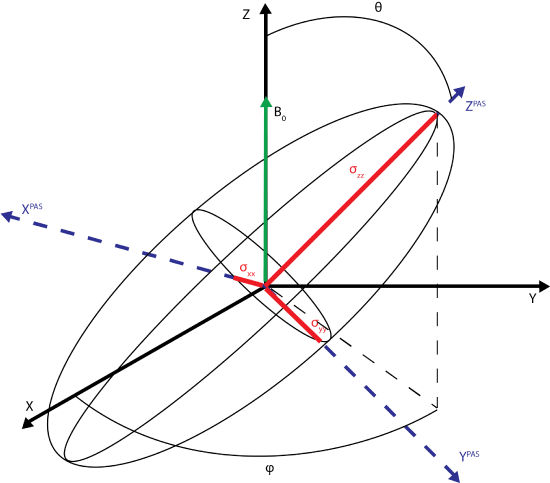
\includegraphics[width=0.4\linewidth]{Figures/Chemical_Shift_Tensor.png}
  \caption[Principal axis system with respect to laboratory reference.]{Representation of the principal axis system (PAS, blue dotted lines) with respect to the laboratory reference frame (black solid lines). The polar angles $\theta$ and $\phi$ relate the former to the latter. The principal components of the tensor are shown in red, and the overall shape is shown by the black ellipses.}
  \label{fig:chemical-shielding-tensor}
\end{figure}

In almost all experiments, the chemical shielding tensor $\sigma$ is only indirected measured, via the chemical shift $\delta$, which is defined with respect to a reference nucleus such that $\delta = \sigma_{\textrm{ref}} - \sigma_{\textrm{sample}}$.
As the coordinate system as described above is somewhat arbitrary, the IUPAC convention defines the three principal components of the chemical shift tensor $\delta_{11}$, $\delta_{22}$ and $\delta_{33}$ such that $\delta_{11} \geq \delta_{22} \geq \delta_{33}$.
The isotropic chemical shift is given by the average $\delta_{\textrm{iso}} = \frac{(\delta_{11} + \delta_{22} + \delta_{33})}{3}$.
There are two other conventions for describing chemical shift anisotropy, which are useful in different contexts.
The Herzfeld Berger convention represents the chemical shift in terms of the span of the signal $\Omega = \delta_{11} - \delta_{33}$ and the skew $\kappa = \frac{3(\delta_{22} - \delta_{\textrm{iso}})}{\Omega}$ where $\delta_{\textrm{iso}}$ is the same as in the IUPAC convention.
This is particularly useful for intuitively describing the powder lineshape formed by a given signal.
The other convention is the Haeberlen convention, which defines the three principal components as $|\delta_{zz} - \delta_{\textrm{iso}}| \geq |\delta_{xx} - \delta_{\textrm{iso}}| \geq |\delta_{yy} - \delta_{\textrm{iso}}|$, and the parameters $\delta = \delta_{zz} -\delta_{\textrm{iso}}$ and $\eta = \frac{\delta_{xx} - \delta_{yy}}{\delta_{zz} -\delta_{\textrm{iso}}}$.
This convention is most useful for describing the angular dependence of a chemical shift on the polar angles $\theta$ and $\phi$, which is given by the relationship\autocite{Haeberlen1976}
\begin{equation}
  \delta_{\textrm{obs}} = \delta_{\textrm{iso}} + \delta \left(\frac{3 \cos^2 \theta - 1 + \eta \sin^2 \theta \cos 2 \phi}{2} \right)
  \label{eqn:orientation-csa}
\end{equation}

In a non-spinning polycrystalline or amorphous powder, the above expression can be integrated over the range of chemical shifts to give the characterisitc powder lineshape see in \cref{fig:ssnmr-tensor}, reproduced from the work of Facelli, Grant, and Michl.\autocite{Facelli1987Carbon-13Determination}
The sample consists of randomly oriented tensors, all of which contribute to the signal.
The principal values of the tensor $\delta_{11}$, $\delta_{22}$ and $\delta_{33}$ correspond to the two extrema of the line, and the central peak.

\begin{figure}
  \centering
  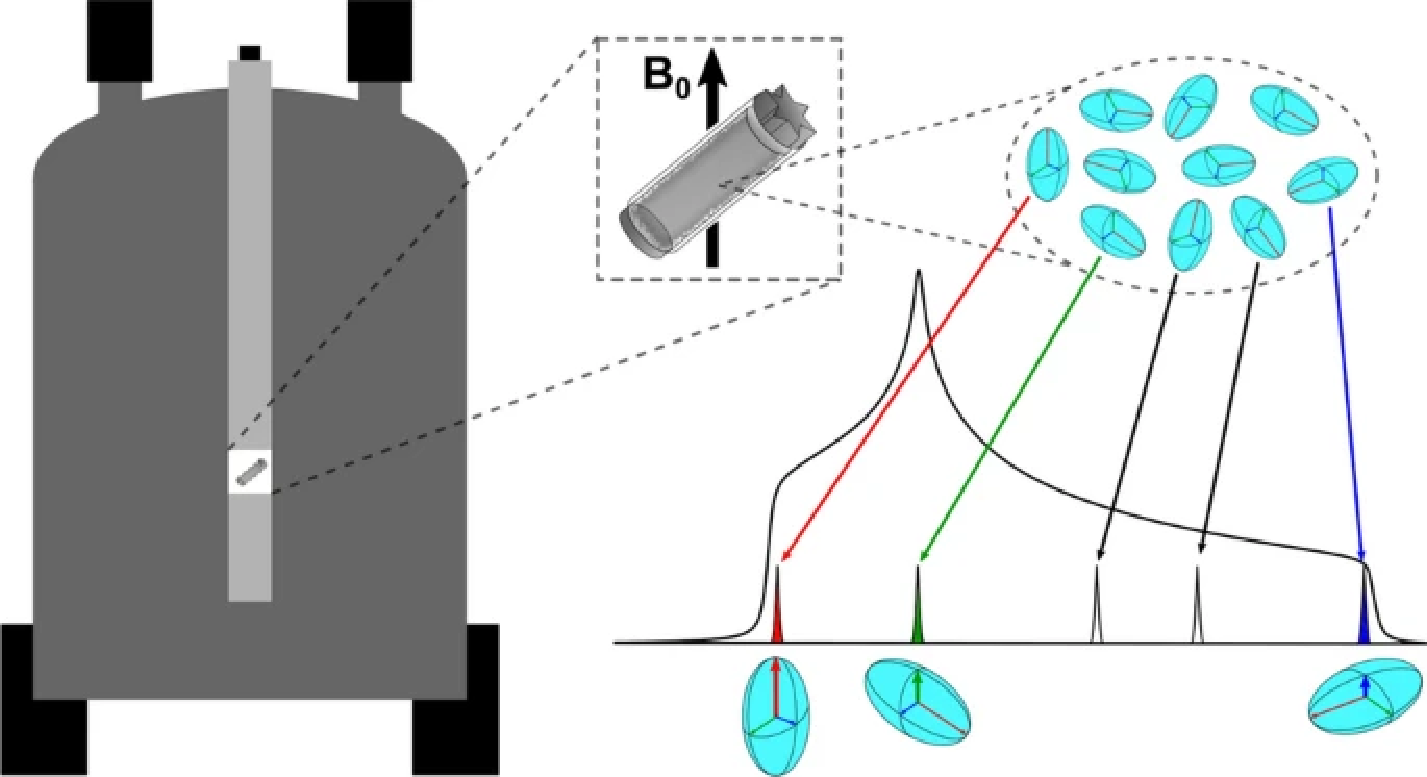
\includegraphics[width=0.45\linewidth]{Figures/ssnmr-tensor.pdf}
  \caption[SSNMR powder lineshape]{Characteristic solid-state NMR powder lineshape for an asymmetric tensor e.g. in an alkene. The positions of the three principal values are shown.}
  \label{fig:ssnmr-tensor}
\end{figure}

The extremely poor S/N ratio (especially for a relatively insensitive nucleus like \ce{^{77}Se}) limits the utility of this method, as the radiated signal from the nuclei is spread out over a large bandwidth.
Spinning at the magic angle can improve the S/N ratio by partially averaging out the chemical shift anisotropy and dipolar relaxation.
Instead of the powder pattern, we instead observe a sharp isotropic chemical shift and a series of spinning sidebands which are separated from the isotropic peak by multiples of the spinning frequency.
The radiated power is thus concentrated in narrower bands, leading to a much improved S/N ratio.

An example is presented in \cref{fig:31P-ssnmr} of proton decoupled solid state \ce{^{31}P} spectra of barium diethyl phosphate, reproduced from the work of Herzfeld and Berger\autocite{Herzfeld1980SidebandAngle}.
In the first spectrum, no magic angle spinning was used, and the lineshape is characteristically broadened into an asymmetric peak (the powder lineshape).
Note the poor S/N ratio due to the broad peak.
The S/N ratio can be seen to improve as the spinning speed increases, and the sidebands become more sparse, affording a stronger signal overall.

\begin{figure}
    \centering
    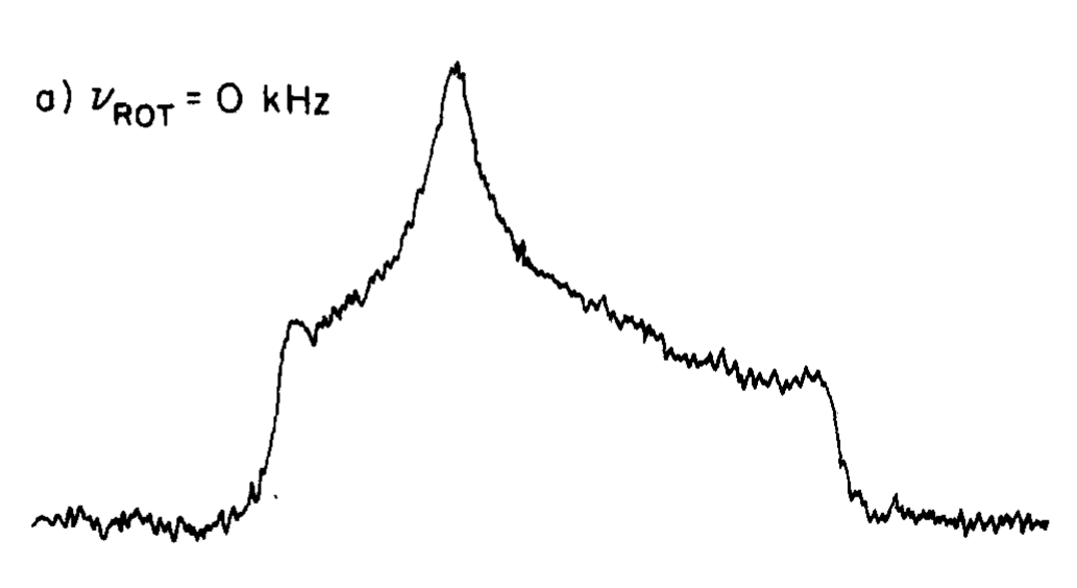
\includegraphics[width=0.45\linewidth]{Figures/31P-ssnmr-0khz.pdf}
    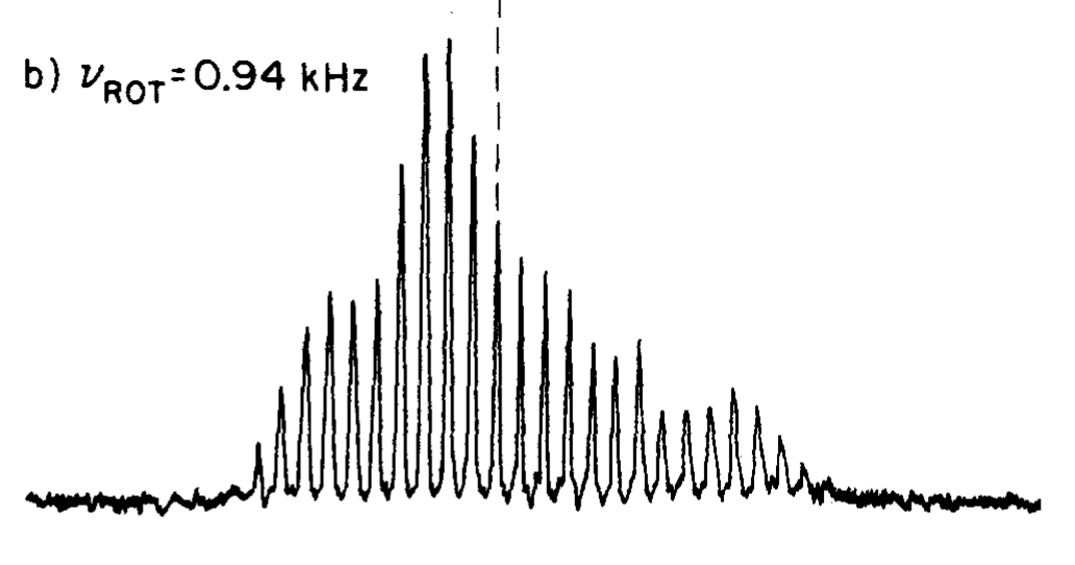
\includegraphics[width=0.45\linewidth]{Figures/31P-ssnmr-0.94khz.pdf}

    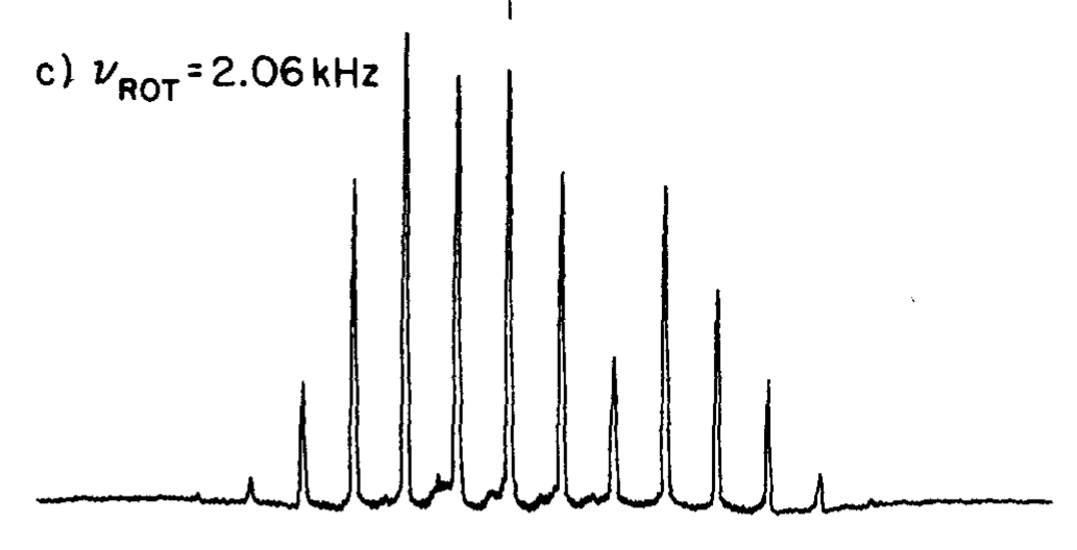
\includegraphics[width=0.45\linewidth]{Figures/31P-ssnmr-2.06khz.pdf}
    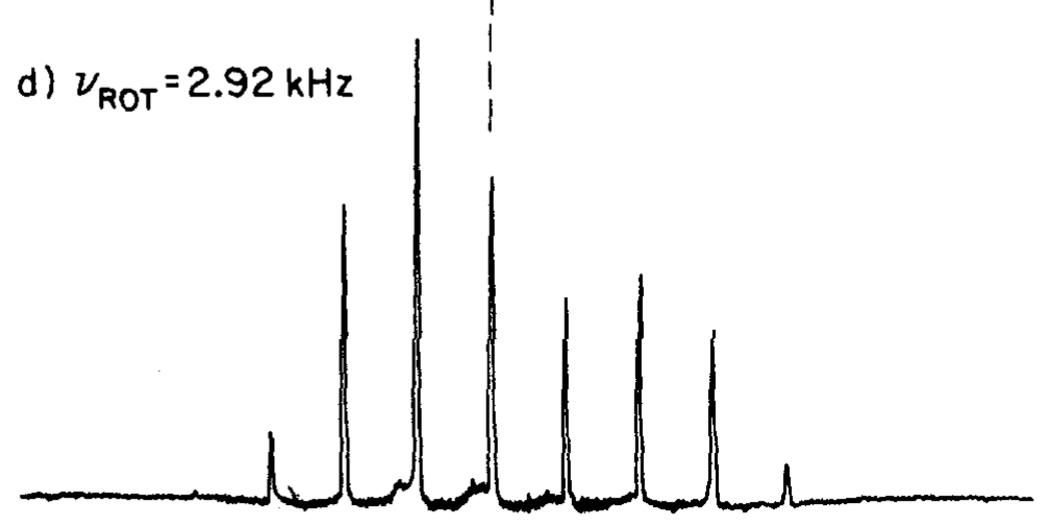
\includegraphics[width=0.45\linewidth]{Figures/31P-ssnmr-2.92khz.pdf}
    \caption[31P SSNMR spinning at the magic angle.]{Proton decoupled solid state \ce{^{31}P} spectra of barium diethyl phosphate spinning at the magic angle, at the speed specified. The isotropic chemical shift is shown by the vertical dotted line.}
    \label{fig:31P-ssnmr}
\end{figure}

The principal values of the tensor are clearly easily obtained from a non-spinning sample, as they can practically be read off the spectrum.
However, the extremely poor S/N ratio (especially for a relatively insensitive nucleus like \ce{^{77}Se}) limits the utility of this method.
Spinning at the magic angle is clearly necessary to improve the S/N ratio, however this obscures the true locations of the extrema of the signal, therefore the values of $\delta_{11}$ and $\delta_{33}$, as well as modifying the position of the maximum ($\delta_{22}$).

There exist programs (such as SOLA, integrated within TopSpin by Bruker BioSpin) which can fit an experimental lineshape or sideband manifold affording the principal values of the tensor, however there is clearly a trade-off between obtaining a good S/N ratio and having enough sidebands within the limits of the signal for a meaningful fit.
Another issue is encountered with preferred orientation of crystallites, as in powder diffraction, which is not modelled in the fitting routine, leading to a poorer fit.
Perhaps the most fundamental issue stems from the fact that the sample is a powder of randomly oriented particles.
This means that the absolute orientation of the tensor with respect to the molecule cannot be determined from this kind of experiment.
Nonetheless, the \emph{shape} of the tensor is still valuable information that may be able to shed light on Ch-bonding in the solid phase.

\printbibliography[heading=subbibliography]
\end{refsection}

\begin{refsection}

\chapter[Simulating chalcogen bonding using molecular mechanics]{Simulating chalcogen bonding using molecular mechanics: A pseudoatom approach to model ebselen.}

This chapter was submitted to \textit{chemRxiv}, 21 Mar 2020.\autocite{Fellowes2020chemrxiv}

\section{Abstract}
The organoselenium compound ebselen has recently been investigated as a treatment for COVID-19, however efforts to model ebselen \emph{in silico} have been hampered by the lack of an efficient and accurate method to assess its binding to biological macromolecules. We present here a Generalized Amber Force Field modification which incorporates classical parameters for the selenium atom in ebselen, as well as a positively charged pseudoatom to simulate the $\sigma$-hole, a quantum mechanical phenomenon that dominates the chemistry of ebselen. Our approach is justified using an energy decomposition analysis of a number of DFT optimized structures, which show that the $\sigma$-hole interaction is primarily electrostatic in origin. Finally, our model is verified by conducting MD simulations on a number of simple complexes, as well as the clinically relevant enzyme SOD1, which is known to bind to ebselen.

\section{Introduction}
Ebselen (\cmpd{ebs}) is a molecule that has piqued the interest of many medicinal chemists, in no small part due to its decidedly non-druglike appearance.
First synthesized in 1924, its unusual properties went more or less uninvestigated for more than 50 years.\autocite{Lesser1924}
Interest in ebselen boomed in the early 1980s, and since then it has been the subject of several studies into its synthesis, biological properties, and metabolism.\autocite{Weber1976,Renson1981,Muller1984,Wendel1984,Parnham1984,Engman1989,Schewe1995,Bhabak2010,Iwasaki2017}
Its biological activity can be broadly attributed to its ability to neutralize reactive oxygen species (ROS), reducing the level of oxidative stress to which cells are subjected.\autocite{Mugesh2000}
To this end, ebselen has been investigated for its neuroprotective, mood-stabilizing, anti-inflammatory, and anti-cancer properties.\autocite{Parnham1987,Kil2007,Singh2013,Azad2014,Parnham2000,Chantadul2020}
Recently it was identified as a compound of interest for the treatment of COVID-19, showing promising inhibition of the viral M\textsuperscript{pro} protease enzyme.\autocite{Jin2020}

The \emph{in vivo} antioxidant ability of ebselen is believed to be mediated through a catalytic cycle analogous to that of glutathione peroxidase (a selenoenzyme).\autocite{Antony2011}
The selenium-containing heterocycle is reductively opened to afford the free selenol, which is the active catalyst.
This is rapidly oxidised by ROS to a selenenic acid, which is then reduced back to the selenol by glutathione (GSH) via a selenenyl sulfide (\cref{fig:catcycle}).
Its activity against a number of other targets appears to also be mediated through formation of a covalent complex via nucleophilic attack at the selenium.
There is also evidence that ebselen interacts with targets non-covalently.\autocite{Jin2020}
These interactions may include association with aromatic or hydrophobic residues, or H-bonding through the carbonyl.
Ebselen can also form non-covalent complexes with Lewis bases through an electrophilic $\sigma$-hole on the selenium atom, similarly to electron-deficient sulfur-containing molecules.\autocite{Thomas2015,Fellowes2019,Beno2015}

\begin{figure}
\centering
\replacecmpd{ebs}
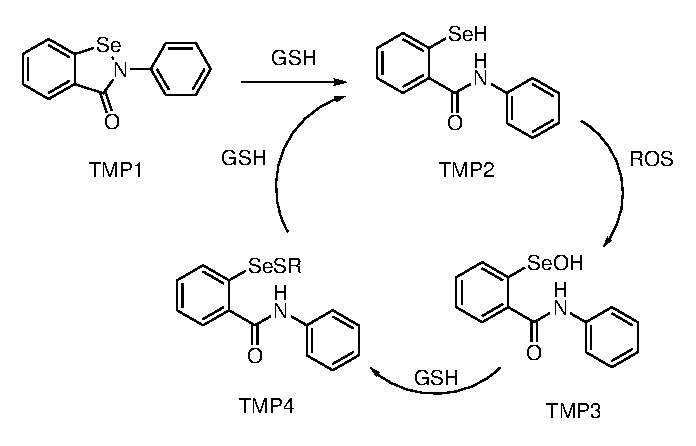
\includegraphics[scale=0.74]{Figures/ebs-cat-cycle.eps}
\caption{Catalytic cycle of ebselen \refcmpd{ebs} \emph{in vivo}.}
\label{fig:catcycle}
\end{figure}

Molecular modelling is a vital tool in drug development, allowing for rapid and broad-reaching screening of drug candidates against likely substrates at minimal cost and risk.
\emph{Ab initio} quantum methods (QM) are widely used to model small molecules (generally smaller than a few hundred atoms), where their accuracy and ability to describe quantum effects underlying photochemical properties and bond breaking/formation processes are critical.
They are however, computationally costly.
Molecular mechanics (MM), where systems are treated strictly classically, is a viable alternative for large systems.
The drawbacks are that MM relies on having an extensive parameter set (a ``force field'') to describe the system (which is not necessarily available, or applicable to the system at hand), and that descriptions of quantum effects often fail spectacularly.

Both of these issues are encountered when attempting to model ebselen using MM.
Firstly, parameters to describe selenium-containing small molecules are simply not available in most popular force fields, including GAFF, Gromos, and CGenFF.
This has been substantially addressed in the work of Torsello et al., where extensive parametrization of a series of diaryl diselenides and diaryl ditellurides was performed, and they provided a methodology to extend this to general chalcogen-containing molecules.\autocite{Torsello2016}
They did not, however, address the second issue of quantum effects, which is reasonable given that they do not play a large role in diselenides.
The chemistry of ebselen, on the other hand, is dominated by the $\sigma$-hole, which is a quantum effect.\autocite{Thomas2015}
The $\sigma$-hole is a region of positive electrostatic potential situated opposite to the Se--N bond, caused by a strongly anisotropic electron distribution around the selenium atom.
This causes the selenium to adopt a highly directional electrophilic character, which can lead to the formation of ``chalcogen-bonds'' with electron pair donors (named by analogy to the ubiquitous hydrogen bond).\autocite{Murray2009}

The presence of a $\sigma$-hole is not a new problem in MM, nor are they exclusive to chalcogens, as they are also found on the heavier halogens, where they give rise to halogen bonding.\autocite{Clark2007}
Perhaps due to the higher prevalence of halogens in drug-like molecules, a number of approaches have been proposed to account for $\sigma$-holes in halogenated molecules.
The common theme in these methods is the inclusion of a pseudoatom with positive electrostatic potential attached to the halogen atom.
This pseudoatom is variously called an extra point (EP), explicit $\sigma$-hole (ESH), or virtual or off-atom centered point, and the approaches differ in the location of the pseudoatom and method used to derive its charge.\autocite{Renidine2011,Ibrahim2011,Hobza2012,Harder2016}
Lone pairs can also be described using negatively charged pseudoatoms, and this approach has been used for some time.\autocite{Dixon1997,Cieplak2001,Harder2016}

It is worth noting an alternative approach, used by Cozzolino and Vargas-Baca, which treats secondary bonding interactions as true bonds, with an explicitly parametrized potential.\autocite{Cozzolino2011}
This was used to parametrize the supramolecular synthon 1,2,5-tellura\-dizaole, which is known to self assemble into a range of interesting structures.
This approach, however, relies on describing the bond using an \emph{an}harmonic potential, which is not easily implemented in most software.

The inability to model ebselen in biological systems is a major hurdle in understanding the mechanism of its action.
Furthermore, recent high-profile work has highlighted the need for an accurate force field which takes quantum effects into account.\autocite{Weglarz-Tomczak2021,Menendez2020}
In this work we develop a parameter set for the selenium atom in ebselen, including a pseudoatom to simulate the $\sigma$-hole.
We have based the force field on GAFF, due to its popularity and ability to describe most druglike molecules in a way which is compatible with biomolecular force fields.
Although GAFF is designed to work in the AMBER molecular dynamics system, we used GROMACS to develop the parameters, as it natively supports massless pseudoatoms which were critical for the description of the $\sigma$-hole.
In principle, the work could be translated to any program that supports massless points, or the pseudoatom could even be given a mass and associated harmonic parameters which would enable some level of polarisability.
However we have simply provided the GROMACS parameters with the massless point for its numerical stability and speed.
Using these parameters, we show that this model accurately reproduces experimental geometries and energies, and compares favourably to \emph{ab initio} calculations.
This force field will prove useful in understanding the interactions between ebselen and current targets, and possibly lead to the discovery of new targets.

\section{Results and Discussion}
We began by deriving the classical bonding parameters involving selenium in ebselen, using the procedure of Torsello.\autocite{Torsello2016}
All quantum calculations were performed using Gaussian16, unless otherwise specified.\autocite{gaussian16}
Electrostatic potentials were calculated using the \texttt{cubegen} program in the Gaussian suite, or \texttt{mol2cub}.\autocite{mol2cub}
The ground state geometry of ebselen was optimized at the $\omega$B97M-V/def2-TZVP level, followed by vibrational analysis to confirm the structure was minimized.\autocite{Chai2008,Weigend2005,Weigend2006}
The range-separated hybrid functional $\omega$B97M-V has been shown to accurately describe Ch-bonding interactions at modest computational cost.\autocite{Mehta2021}
Partial charges were assigned to the atoms using the RESP scheme, at the HF/6-31G* level.\autocite{Cornell1993}
This was chosen for consistency with existing AMBER force fields.

\subsection{Classical bonding parameters}
Bond and angle force constants were derived by conducting a relaxed potential energy surface scan over a range of $\pm0.3$~\AA~for bonds and $\pm10$\degree~for angles.
The resulting data was truncated to within 5~kcal/mol of the equilibrium energy (at larger distances the surfaces were appreciably anharmonic), and this surface was fitted with a classical harmonic oscillator model (\cref{eqn:cho}) using the \texttt{nls} function in the R software package.\autocite{R}
The equilibrium distance/angle $x_0$ was fixed to the value from the optimized geometry.
The resulting potential energy surfaces and harmonic approximations are shown in \cref{fig:pes}.
Torsion angles were similarly scanned at the DFT and MM (with the torsion term set to zero) levels, and the difference between these surfaces was fitted using a periodic series (\cref{eqn:dihe}).
The resulting parameters are presented in \cref{tab:cho-params,tab:dihe-params}.

\begin{equation}
    V(x) = \frac{1}{2} k (x - x_0) ^2
    \label{eqn:cho}
\end{equation}

\begin{equation}
    V(\phi) = \sum_{n=1} \left( \frac{V_{\mathrm{max},n}}{2} \times (1 + \cos(n \phi + \gamma_n)) \right)
    \label{eqn:dihe}
\end{equation}

\begin{table}
    \centering
\begin{tabular}{lll}\toprule
         Parameter & $x_0$ & $k$  \\\midrule
         r(\ce{Se-N}) & 1.8586 & 434.67 \\
         r(\ce{Se-C}) & 1.8829 & 422.33 \\
         $\angle$(\ce{C-Se-N}) & 86.6 & 610.7 \\
         $\angle$(\ce{Se-N-C_{ar}}) & 119.6 & 182.7 \\
         $\angle$(\ce{Se-N-C_{CO}}) & 115.8 & 404.5 \\
         $\angle$(\ce{C-C-Se}) & 119.4 & 329.2 \\
         \bottomrule
    \end{tabular}
    \caption[Classical bonding parameters for ebselen.]{Classical bonding parameters for ebselen. Bond lengths are given in \AA, and angles in degrees. Force constants are given in kcal/mol$\cdot$\AA$^2$ or kcal/mol$\cdot$radian$^2$.}
    \label{tab:cho-params}
\end{table}

\begin{table}
    \centering
    \footnotesize
    \begin{tabular}{lllll}\toprule
         Parameter & $V_\mathrm{max,1}$ & $V_\mathrm{max,2}$& $\gamma_1$ & $\gamma_2$ \\
         & kcal/mol & kcal/mol & \degree & \degree\\\midrule
         $\phi$(\ce{C_{ar}-C_{ar}-N-Se}) & $-0.9653$ & $0.5108$ & 180 & 180 \\
        \bottomrule
    \end{tabular}
    \caption{Dihedral parameters for ebselen.}
    \label{tab:dihe-params}
\end{table}

\begin{figure}
    \centering
    \begin{subfigure}{0.4\linewidth}
        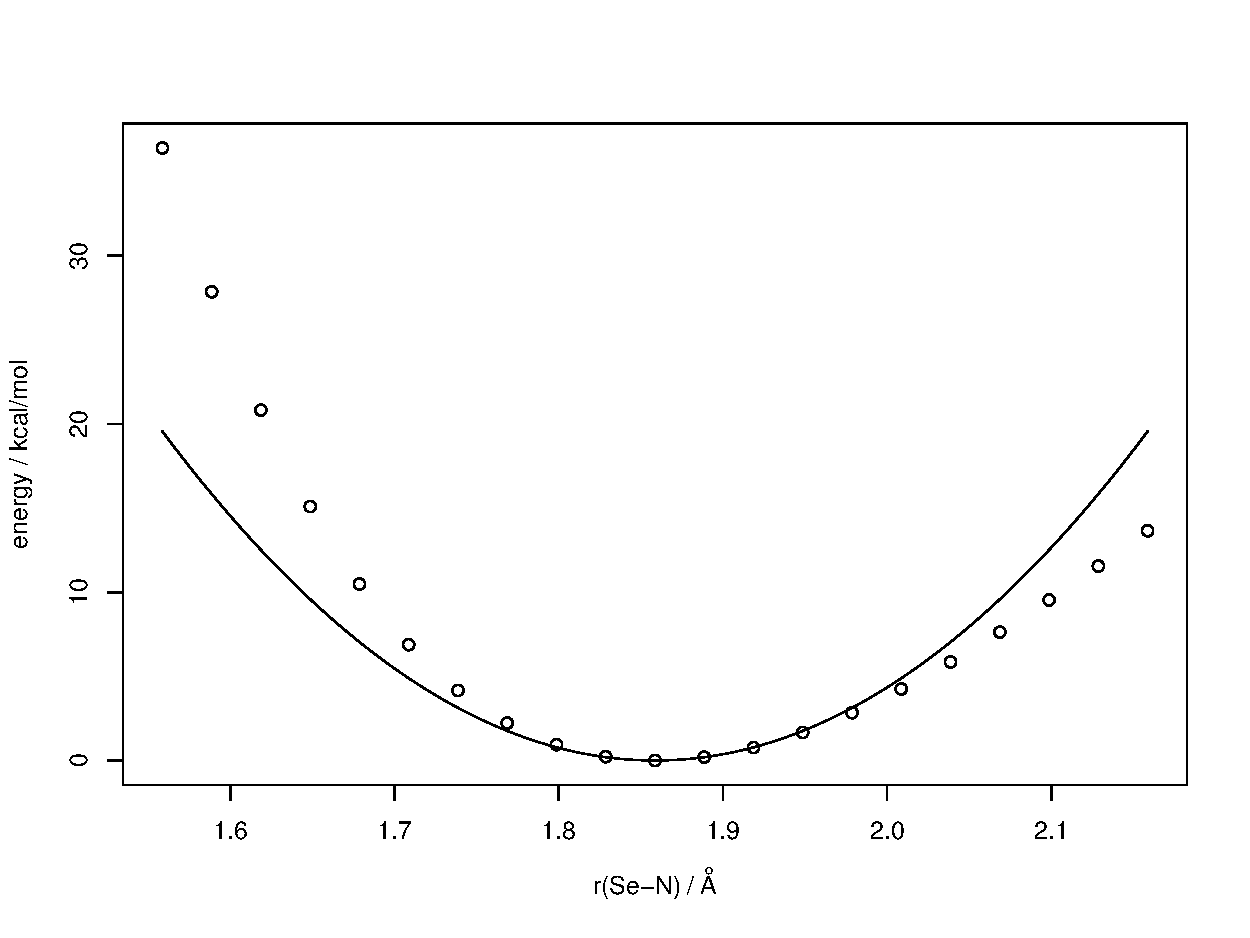
\includegraphics[width=\linewidth]{Figures/ch2-sifig/SeN.pdf}
        \caption{r(\ce{Se-N})}
    \end{subfigure}
    \begin{subfigure}{0.4\linewidth}
        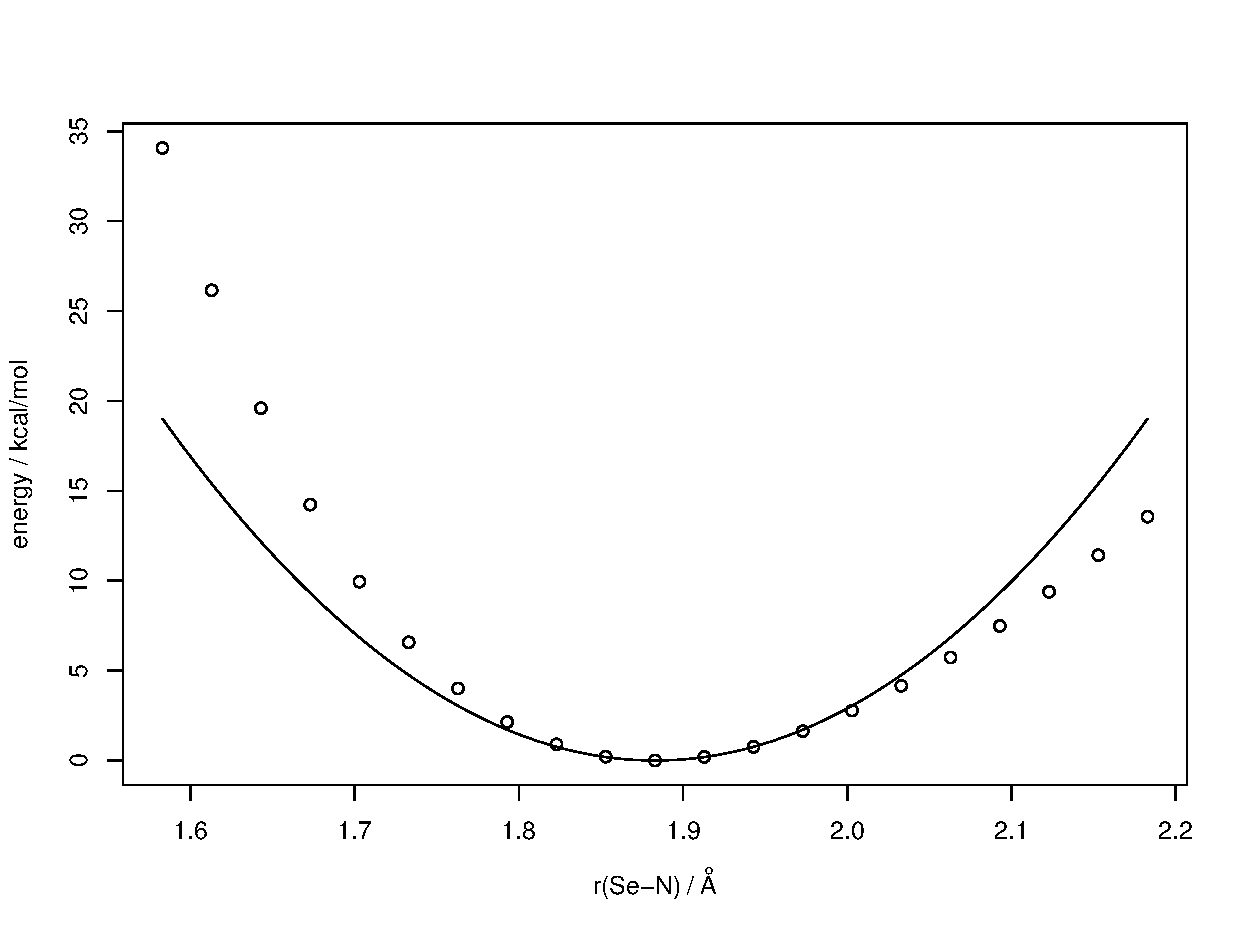
\includegraphics[width=\linewidth]{Figures/ch2-sifig/SeC.pdf}
        \caption{r(\ce{Se-C})}
    \end{subfigure}
    \begin{subfigure}{0.4\linewidth}
        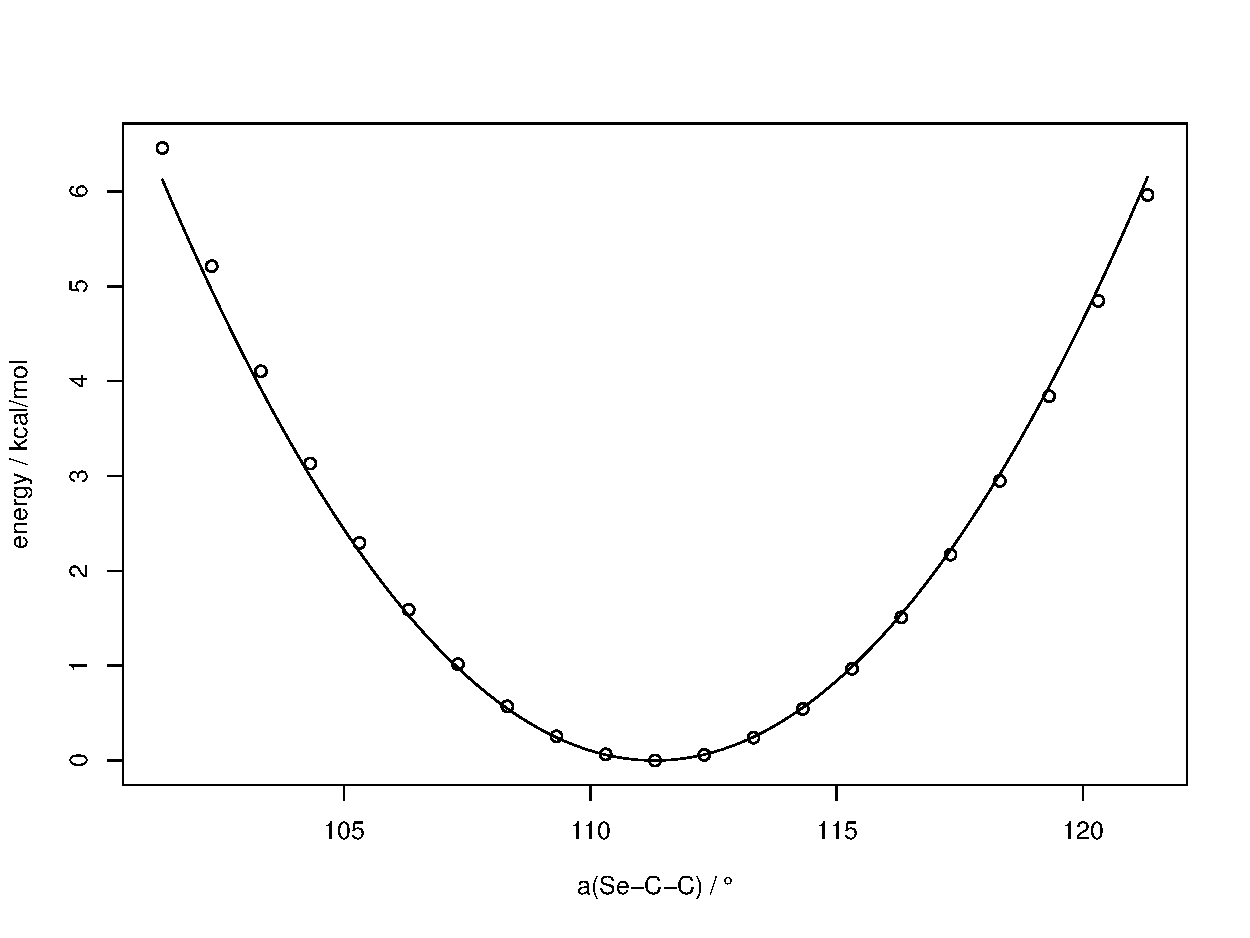
\includegraphics[width=\linewidth]{Figures/ch2-sifig/SeCC1.pdf}
        \caption{$\angle$(\ce{Se-C_1-C_6})}
    \end{subfigure}
    \begin{subfigure}{0.4\linewidth}
        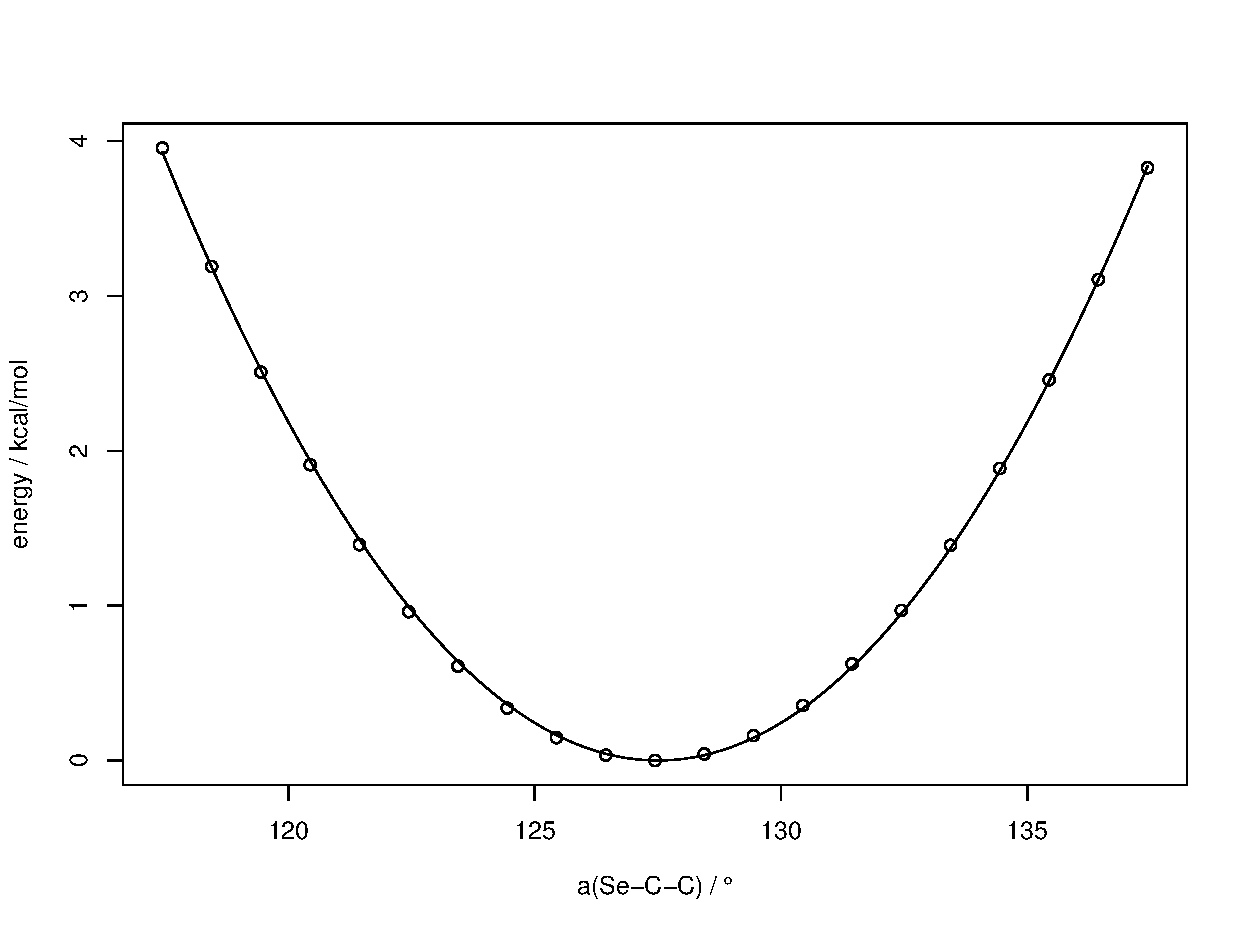
\includegraphics[width=\linewidth]{Figures/ch2-sifig/SeCC2.pdf}
        \caption{$\angle$(\ce{Se-C_1-C_2})}
    \end{subfigure}
    \begin{subfigure}{0.4\linewidth}
        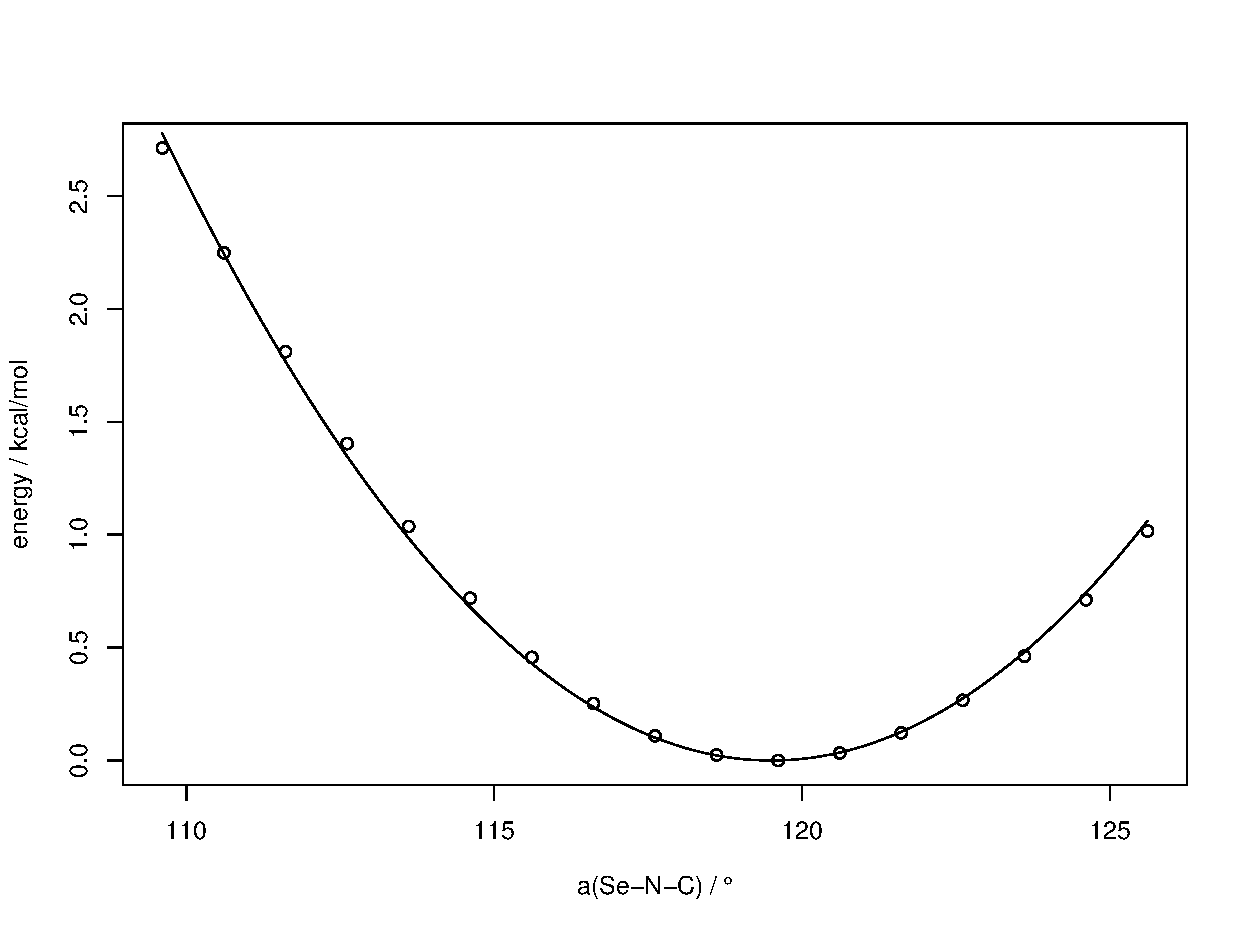
\includegraphics[width=\linewidth]{Figures/ch2-sifig/SeNC1.pdf}
        \caption{$\angle$(\ce{Se-N-C_{8}})}
    \end{subfigure}
    \begin{subfigure}{0.4\linewidth}
        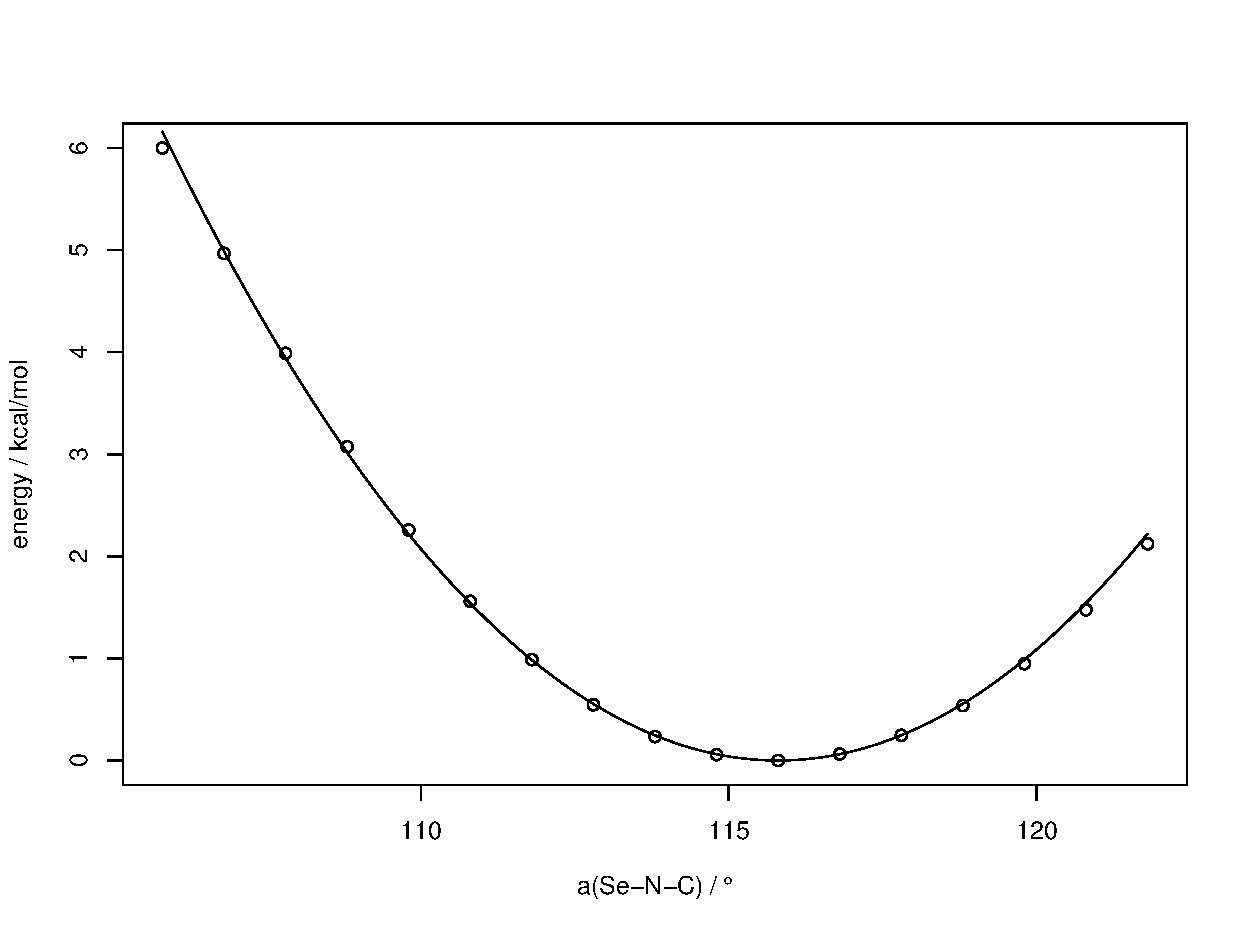
\includegraphics[width=\linewidth]{Figures/ch2-sifig/SeNC2.pdf}
        \caption{$\angle$(\ce{Se-N-C_{7}})}
    \end{subfigure}
    \begin{subfigure}{0.4\linewidth}
        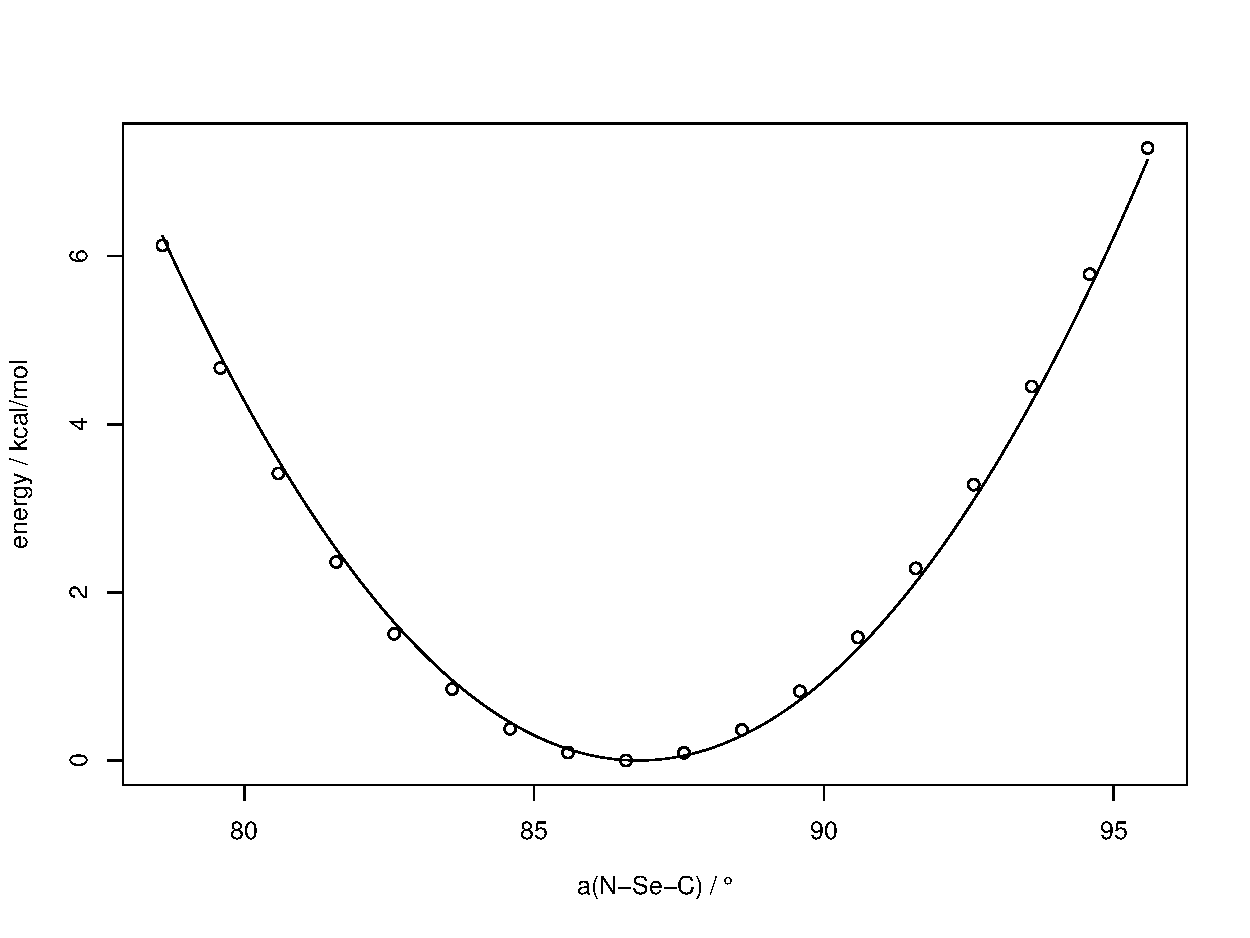
\includegraphics[width=\linewidth]{Figures/ch2-sifig/NSeC.pdf}
        \caption{$\angle$(\ce{N-Se-C})}
    \end{subfigure}
    \begin{subfigure}{0.4\linewidth}
        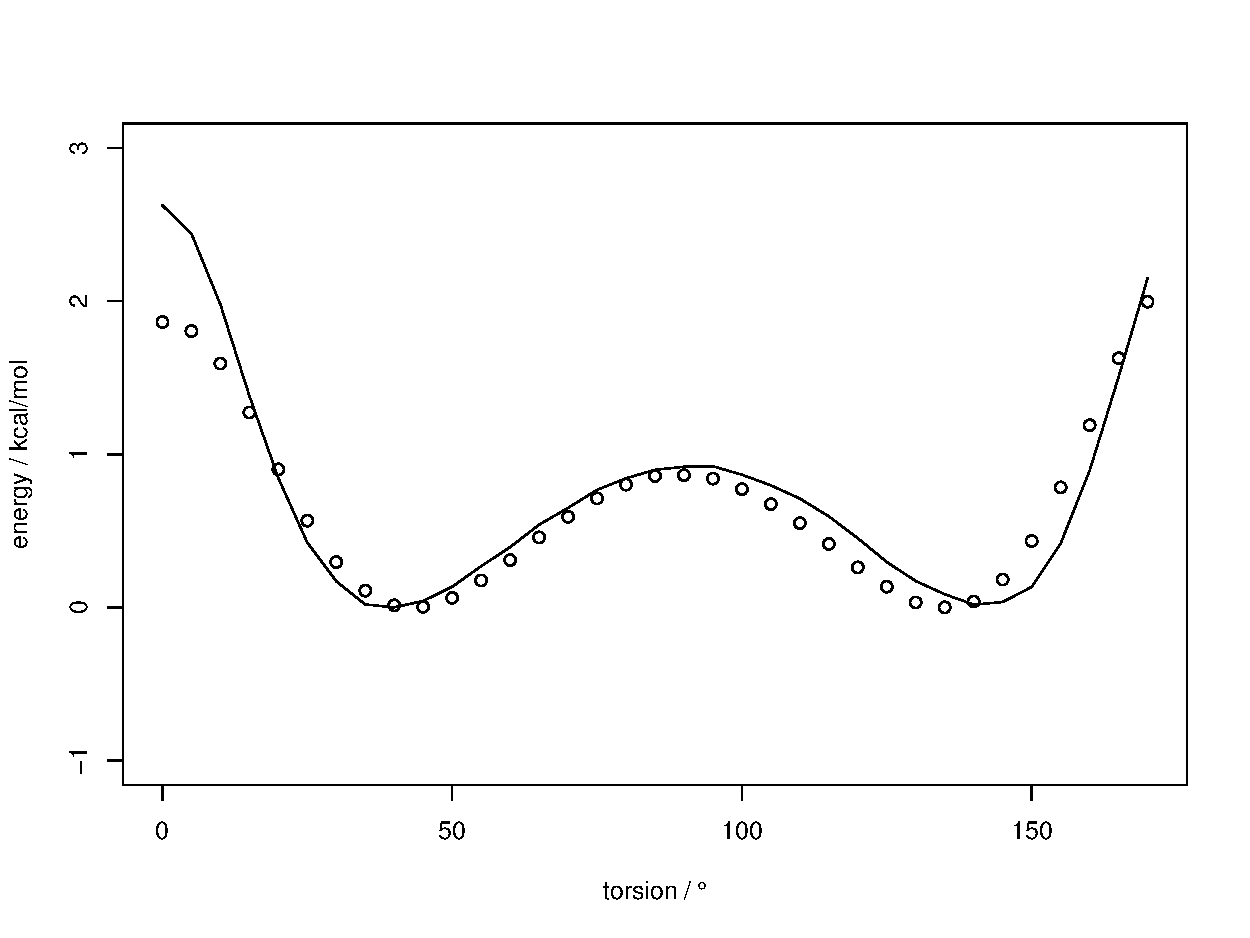
\includegraphics[width=\linewidth]{Figures/ch2-sifig/SeNCC.pdf}
        \caption{$\phi$(\ce{Se-N-C-C})}
    \end{subfigure}
    \caption[Potential energy surfaces of ebselen.]{Potential energy surfaces for the indicated geomeric parameter. The DFT surface is shown as points and the harmonic approximation is shown as a line.}
    \label{fig:pes}
\end{figure}

Values of 2.12 and 0.2910 for the Lennard-Jones parameters $\sigma$ and $\varepsilon$ were used for selenium, to account for the polar flattening that is observed in strongly polarised atoms.
These values are lower than would be expected for a large atom like selenium (e.g. sulfur's parameters are only slightly lower at 1.9825 and 0.2824), however we found that they gave the most realistic bond energies and geometries.
This is likely due to errors in the force field which are cancelled out by these artificially low values, which we believe is acceptable seeing as our goal is to provide an internally consistent system rather than absolute truth. 
The default GAFF Lennard-Jones parameters for the carbonyl oxygen were found to give an unreasonably high barrier to rotation about the central dihedral angle (due to steric repulsion between the oxygen and the aryl hydrogen), so they were changed to 1.5 and 0.08.
This did not appear to have any negative effect on the rest of the model.

Default GAFF values were used for all other atoms, and Lorentz/Berthelot mixing rules were used to derive cross-terms.

\subsection{Energy decomposition analysis}
While attempting to model the $\sigma$-hole using molecular mechanics, we must remember that we are forcing a classical treatment onto an inherently quantum phenomenon.
That said, some parts of the quantum phenomenon are easier than others to treat classically.
There are thought to be three attractive energetic components which contribute to a $\sigma$-hole interaction.
Namely, electrostatics, induction, and dispersion.\autocite{Bleiholder2006,Bleiholder2007,Pascoe2017}
The magnitudes of each component of $\sigma$-hole interactions has been the subject of heated debate in recent years.
For many applications, these disagreements are fairly philosophical and of little consequence, however this is not the case when attempting to model $\sigma$-hole interactions using MM.

The electrostatic component generally refers to the interaction between two static (not distorted by each other) electric fields, which can be graphically represented by visualizing the electrostatic potential surfaces of the donor and acceptor moieties (\cref{fig:ebs-esp}).
This is already treated in MM (for the case of atom centered charges) as a sum of pairwise interactions.
The accuracy of this component is only limited by the resolution of the electrostatic potential; it would appear that a pseudoatom approach could thus adequately describe the $\sigma$-hole.
Dispersion is accounted for empirically within the $r^{-6}$ term of the Lennard-Jones potential.

Issues arise when attempting to model the induction component of the $\sigma$-hole $E_{\mathrm{ind}}$.
This component refers to the redistribution of charge within (polarization) or between (charge-transfer) the donor and acceptor as they approach each other.
Movement of charge is simply not accounted for within the most common AMBER force fields.
This presents a large problem, as charge-transfer drives the strong directionality of $\sigma$-hole interactions, and may account for a significant proportion of their strength.

To ensure that this is not an insurmountable problem for this parametrization, we conducted energy decomposition analyses (EDA) on a variety of complexes containing ebselen.
There are numerous EDA schemes available such as KM-EDA, NEDA, and ALMO, however we chose to use symmetry-adapted perturbation theory (SAPT).\autocite{SAPT2020,Jeziorski1994PerturbationComplexes}
In contrast to several other schemes, SAPT explicitly includes dispersion (as opposed to adding it as an empirical correction), and contains no physically meaningless ``catch-all'' energy term.
The total interaction energy $E_\mathrm{tot}$ is decomposed into an electrostatic component $E_\mathrm{elst}$, an inductive component $E_\mathrm{ind}$ (this incorporates polarization and charge transfer, as they are not distinct phenomena within the SAPT framework), and a dispersive component $E_\mathrm{dis}$.
These attractive forces are balanced by a repulsive exchange component $E_\mathrm{exch}$.

Four Lewis bases were chosen which are representative of those likely to be encountered in biological systems, and which span a wide range of basicity.
Their structures are given in \cref{fig:complexes}.
SAPT(DFT) analyses were conducted using the Psi4 software package on geometries optimized at the $\omega$B97M-V/def2-TZVP level, and the results are shown in \cref{fig:eda}.\autocite{Parrish2017}

\begin{figure}
    \centering
    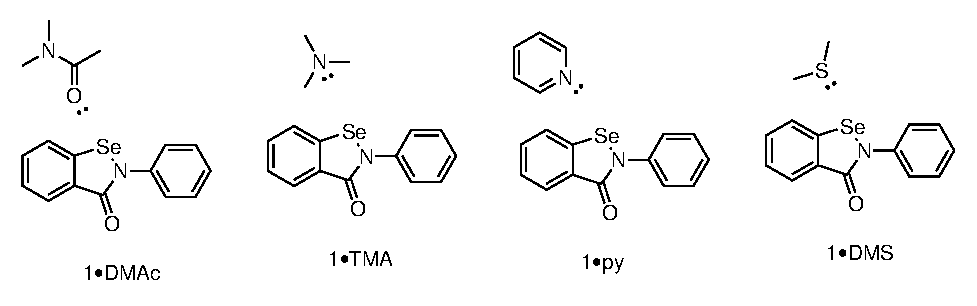
\includegraphics[scale=0.74]{Figures/sapt-complexes.eps}
    \caption{Structures of complexes used for SAPT(DFT) analysis.}
    \label{fig:complexes}
\end{figure}

\begin{figure}
    \centering
    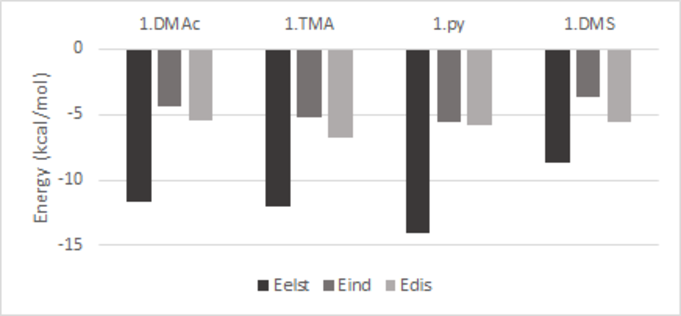
\includegraphics[width=0.75\linewidth]{Figures/sapt-eda.pdf}
    \caption[SAPT(DFT) analysis of complexes with four Lewis bases.]{SAPT(DFT) analysis of complexes with four Lewis bases. All energies are given in kcal/mol.}
    \label{fig:eda}
\end{figure}

The SAPT results indicate that the majority (around 80\%) of the interaction can be described by electrostatics and dispersion.
This suggests that the explicit $\sigma$-hole parametrization will be reliable, as electrostatics and dispersion are well described by MM.

\subsection{Incorporation of pseudoatom}
With classical parameters for ebselen in hand, as well as theoretical assurance that the system can be adequately described using electrostatics, we began to optimize parameters for the pseudoatom representing the $\sigma$-hole.
The pseudoatom was modelled as a virtual site riding on the selenium atom along the extension of the \ce{Se-N} bond.
In GROMACS this is assigned the type \texttt{2fd}, which is described by only one parameter (the distance along the extension of the defining bond).
This is very computationally efficient, although it is an approximation to reality, as the center of the $\sigma$-hole is actually slightly offset (see \cref{fig:ebs-esp}).
A more accurate description would be the three-center \texttt{3fd} or \texttt{3fad} type, however this would introduce a performance penalty.

The distance parameter for the pseudoatom was set to 1.189\AA\ which places the point charge on the VdW surface of the selenium atom.
A number of approaches have been suggested to determine this distance, however it is important for numerical stability of the simulation that the charge lies on or within the VdW surface.\autocite{Hobza2012}
The charge of the pseudoatom was calculated using the RESP procedure, which fits a pre-calculated electrostatic potential to atom- (or pseudoatom-) centered point charges while enforcing symmetry restraints.
The ESP was calculated at the HF/6-31G* level using Gaussian16, in order to be consistent with existing force field parameters.
The pseudoatom was then introduced manually, and RESP applied using the ANTECHAMBER program.
For comparison, we also calculated charges for the structure \emph{without} a pseudoatom.
Relevant charges are presented in \cref{tab:charges}.

\begin{table}
  \centering
    \caption{Selected atomic charges for the pseudoatom and no pseudoatom models.}
    \label{tab:charges}
    \begin{tabular}{lrr}\toprule
        Atom & RESP charge (pseudoatom) & RESP charge (no pseudoatom) \\\midrule
        \ce{E_{26}} & $0.281382$ & --- \\
        \ce{Se_1} & $-0.372631$ & $0.056728$ \\
        \ce{N_2} & $-0.241674$ & $-0.599430$ \\
        \ce{C_3} & $0.463064$ & $0.827981$ \\
        \ce{O_4} & $-0.558076$ & $-0.613468$ \\\bottomrule
    \end{tabular}
\end{table}


\subsection{Electrostatic potential map}
With these parameters in hand, we were able to construct electrostatic potential maps (\cref{fig:ebs-esp}), which show good qualitative agreement between the DFT and pseudoatom model potentials.
Barely visible in the DFT ESP map is a second $\sigma$-hole, opposite the Se--C bond.
Carbon is significantly less electronegative than nitrogen, so it doesn't polarize the selenium to the same degree, leading to a much smaller $\sigma$-hole.
While it is conceivable that this $\sigma$-hole could form Ch-bonds as well, we have not observed any evidence of this in any of the derivatives we have studied.\autocite{Fellowes2019}
We therefore did not attempt to model it, although it could be modelled in the same way as the main $\sigma$-hole opposite the nitrogen.

\begin{figure}
    \centering
    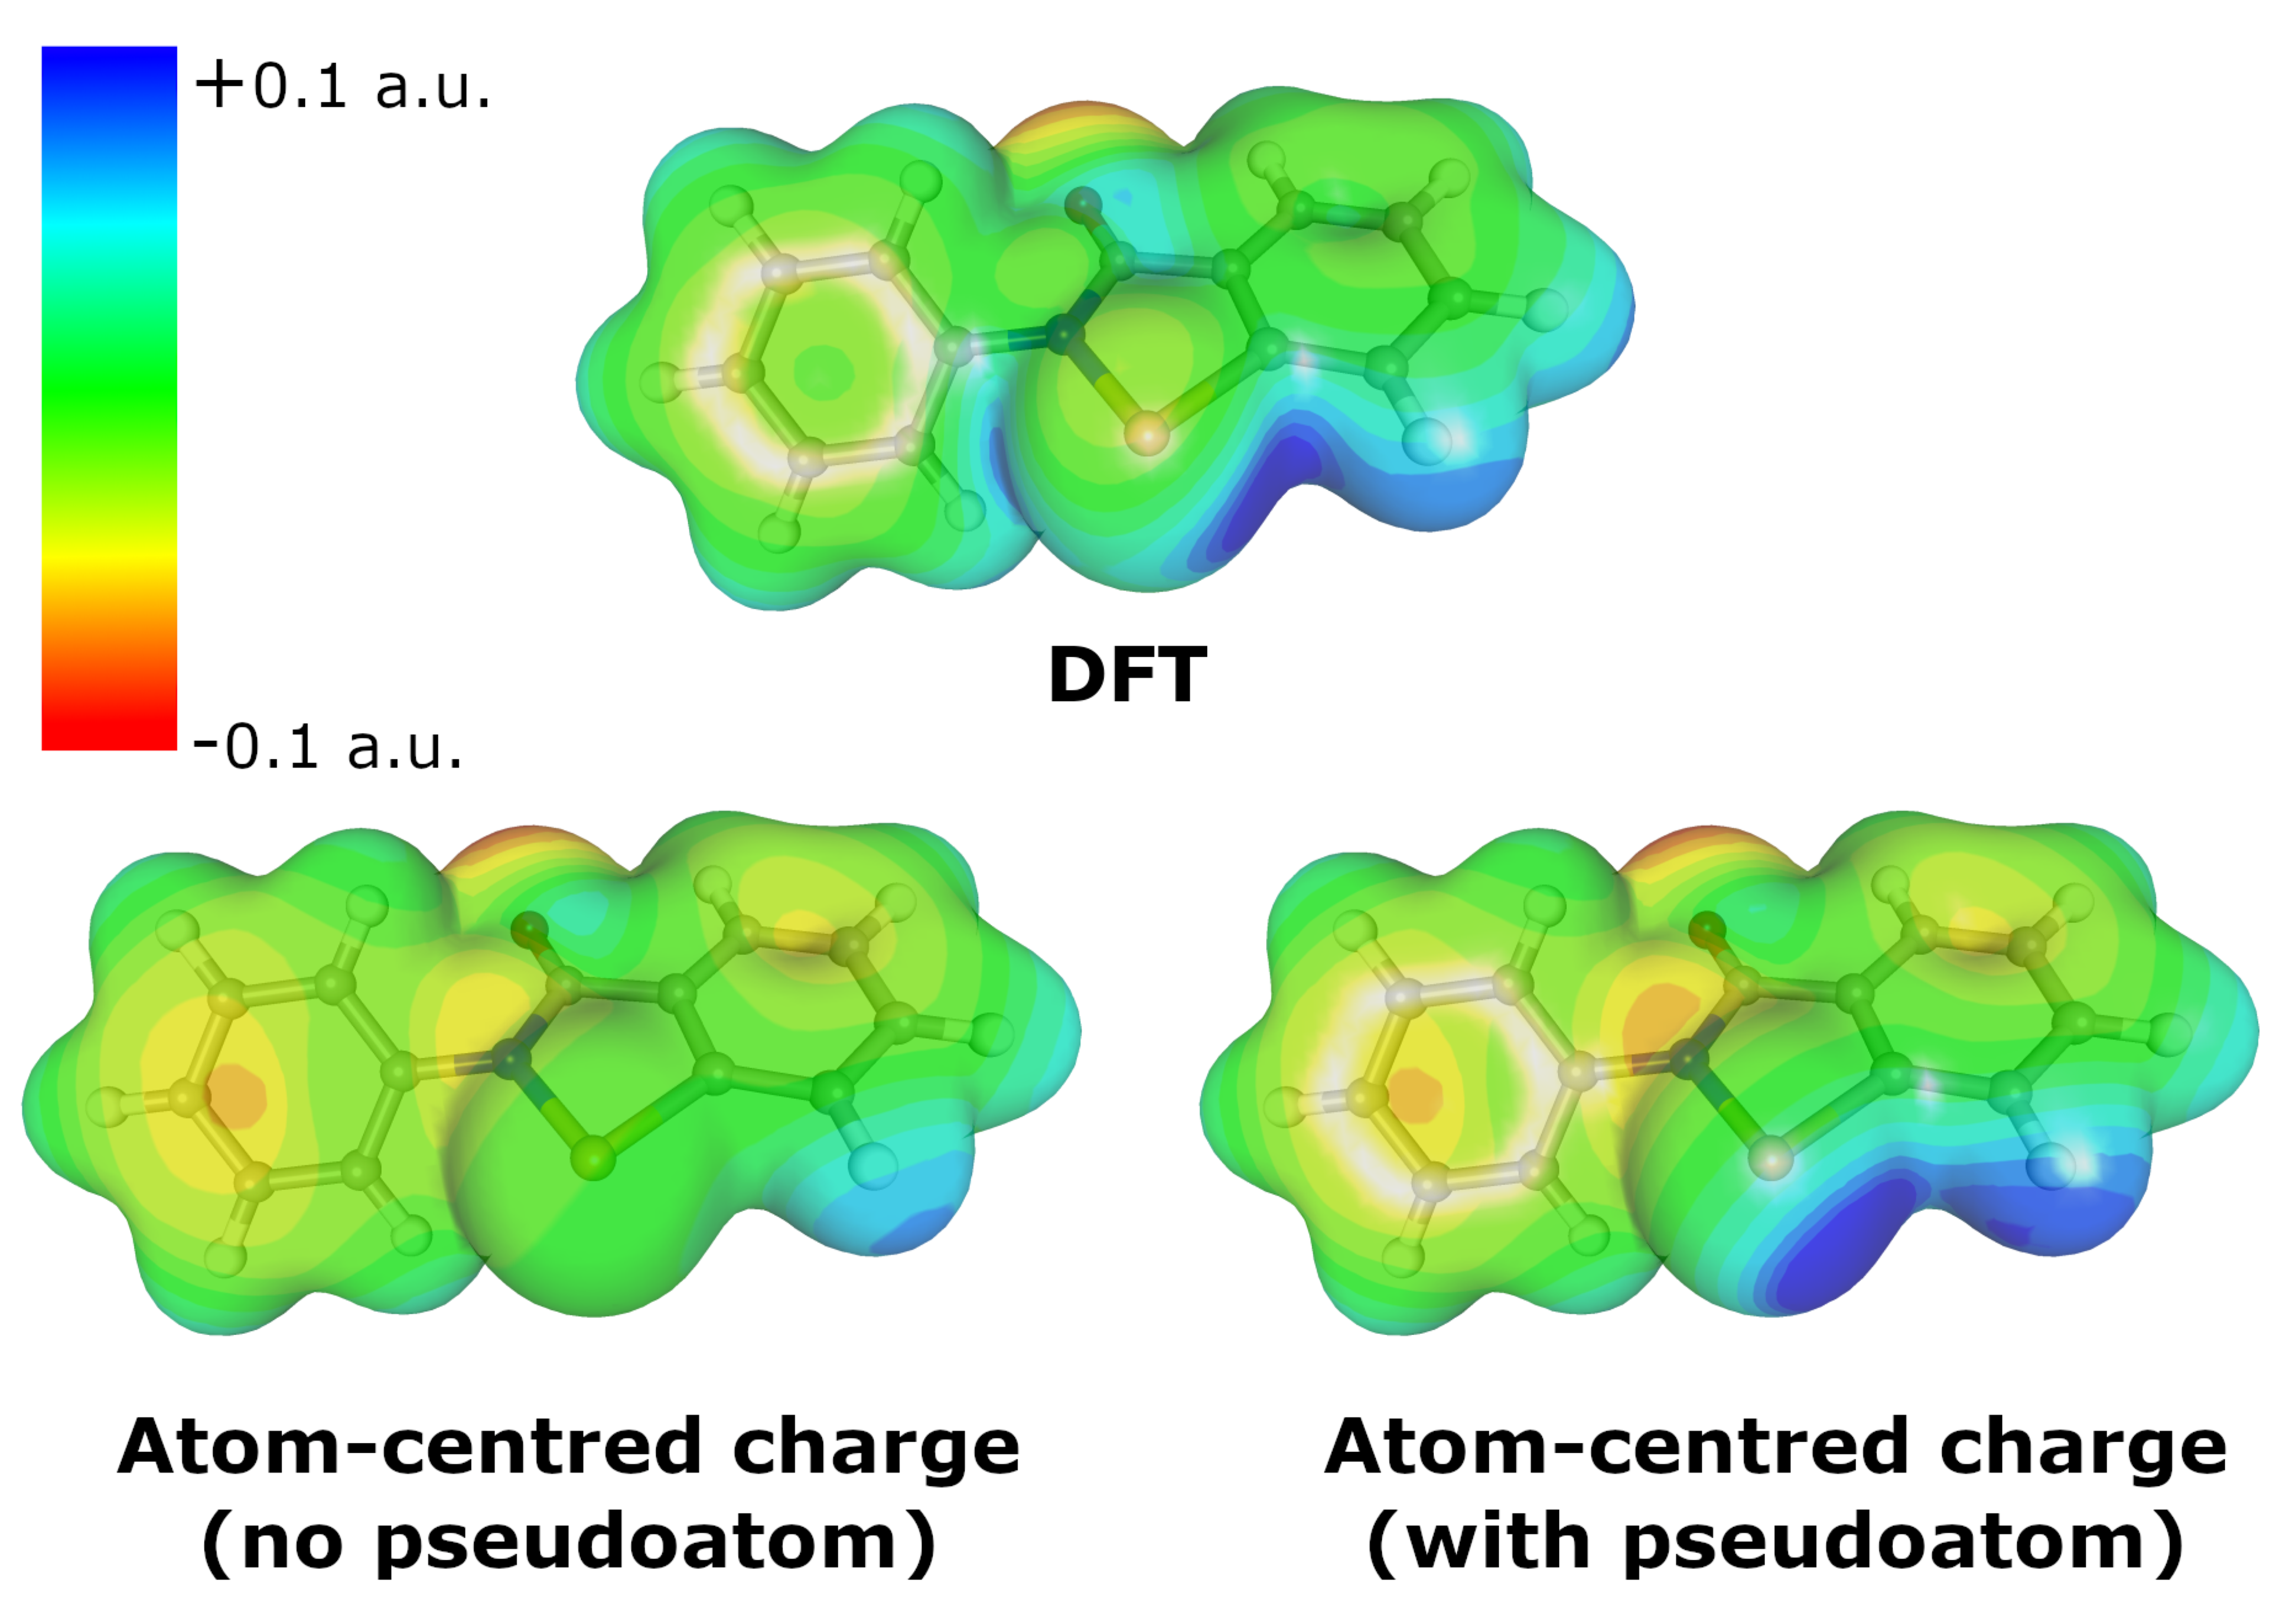
\includegraphics[width=0.5\linewidth]{Figures/mm-dft-esp.pdf}
    \caption[ESP of ebselen generated from DFT density, and atom centred charges.]{ESP mapped on the 0.005~a.u. electron density isosurface. The $\sigma$-hole is visible as the dark blue region on the DFT and atom-centered charge (with pseudoatom) surfaces.}
    \label{fig:ebs-esp}
\end{figure}

\subsection{Validation against DFT geometries}
A preliminary verification of our model was conducted by comparing the geometries and energies calculated in the SAPT(DFT) analysis with the respective MM values.
The Lewis bases chosen for the SAPT(DFT) analysis were constructed in AMBER.
GAFF was used for all atoms, and an extra point was added to simulate the lone pair(s) of the Lewis bases per the method of Dixon and Kollman.\autocite{Dixon1997}
Geometries were assessed by minimizing the ebselen-Lewis base structure, and energies calculated relative to the unbound minimized monomers.
The results are shown in \cref{tab:ebs-geom}.

\begin{table}
    %DONE
    \centering
    \begin{tabular}{lllll}\toprule
        Complex & r(\ce{Se\cdots B}) & $\angle$(\ce{N-Se\cdots B}) & $\angle$(lone pair) & Energy \\ & \AA & \degree & \degree & (kcal/mol)\\\midrule
        \cmpd{ebs}$\cdot$py & 2.879~\AA~(2.775~\AA) & 174.9\degree~(176.2\degree) & 171.1\degree~(165.7\degree) & -7.548 (-7.093) \\%DONE
        \cmpd{ebs}$\cdot$DMAc & 2.741~\AA~(2.786~\AA) & 174.7\degree~(172.4\degree) & 129.1\degree~(117.9\degree) & -7.068 (-7.551) \\%DONE
        \cmpd{ebs}$\cdot$TMA & 2.928~\AA~(2.857~\AA) & 170.1\degree~(177.4\degree) & 107.2\degree~(113.6\degree) & -5.447 (-6.627) \\%DONE
        \cmpd{ebs}$\cdot$DMS & 3.253~\AA~(3.265~\AA) & 160.4\degree~(177.4\degree) & 81.2\degree~(89.8\degree) & -2.510 (-5.646) \\%DONE
        \bottomrule
    \end{tabular}
    \caption[Median geometric parameters for complexes with \refcmpd{ebs}.]{Median geometric parameters for complexes with \refcmpd{ebs}. DFT equilibrium values are given in brackets for comparison. DFT energies are derived from SAPT(DFT).}
    \label{tab:ebs-geom}
\end{table}

These results show that Ch-bonds can be adequately described by the inclusion of a positively charged pseudoatom.
Almost all parameters and energies can be adequately reproduced, with the only anomaly being the substantially underestimated bond energy for the \cmpd{ebs}$\cdot$DMS complex.
Interestingly, the geometry is modelled well in spite of this.
This may be due to the increased role of dispersion in this complex, which has been deliberately de-emphasised in our parameters in order to emulate the polar flattening of the selenium.
There is also a substantial charge-transfer component to this interaction which, when taken to completion, leads to formation of a \ce{Se-S} bond and opening of the ring (\cref{fig:catcycle}).
This cannot be modelled in a harmonic force field, so it is perhaps not surprising that the interaction energy is underestimated.
Nonetheless, we believe that the parameter set will still be very useful for molecular docking.

\subsection{Validation against experimental density}
We also sought to validate our model against the experimentally determined density of the crystal.
An ebselen crystal (CSD code \textbf{SENGOH1}, $5 \times 5 \times 5$ unit cells, 1000 molecules) was constructed, and placed in a simulation box of the appropriate size at 1~atm.
The crystal was heated to 290~K over 2~ns using a Berendsen thermostat and barostat, and the density was calculated to be 1.548~g/cm\textsuperscript{3}, which compares well to the experimental density of 1.529~g/cm\textsuperscript{3} at the same temperature.\autocite{Dupont1990StructuresII}
This procedure was repeated using the non-pseudoatom model, which afforded a density at 290~K of 1.468~g/cm\textsuperscript{3}.
The pseudoatom clearly represents an improvement when simulating the solid state structure of ebselen.

\subsection{Validation against SOD1 binding}
In order to show the utility of our model in a biological context, we conducted a binding simulation with a known ebselen target.
Superoxide dismutase-1 (SOD1) forms a covalent complex with ebselen through the Cys111 residue, which appears to support correct folding of the protein, inhibiting aggregation and associated toxicity.\autocite{Capper2018}
Although formation of the covalent complex cannot be simulated using our model (as this is a bond-forming process), we are able to visualize the stabilized encounter complex which undergoes ring opening to form the final adduct.
Indeed, the Ch-bond formed through the $\sigma$-hole can be thought of as the early stages of a nucleophilic attack at the selenium.\autocite{Thomas2015}
SOD1 (PDB \textbf{2C9V}) was chosen because of the availability of an atomic resolution structure, demonstrated evidence of ebselen binding, and it's relatively small size.\autocite{Capper2018,Strange2006}
The structure was prepared by removing disorder, then removing water and ions (the Cu and Zn ions were retained).
The ff14SB force field was used for the protein.
The ebselen residue was introduced within the binding groove approximately halfway between the two units.
The complex was then neutralized by addition of four \ce{Na+} ions at the sites of most negative electrostatic potential, and solvated with a TIP3P explicit water model to give a final box size of $77.095\times 96.253\times 78.411$~\AA.
The structure was minimized over 1000 cycles to remove bad contacts, then heated to 300~K over 200~ps.
A simulation of 2~ns at 300~K was then performed to assess the average binding geometry, which was found to exhibit a bifurcated Ch-bond between the expected Cys112 sulfur and the adjacent Ile114 backbone carbonyl (\cref{fig:sod1-ebs}).
A similar experiment was performed \emph{without} the $\sigma$-hole, which failed to bind in a reproducible geometry, with the ebselen molecule wandering through the groove.
This is presumably driven by hydrophobic interactions, and the entropic cost of desolvation.

\begin{figure}
    \centering
    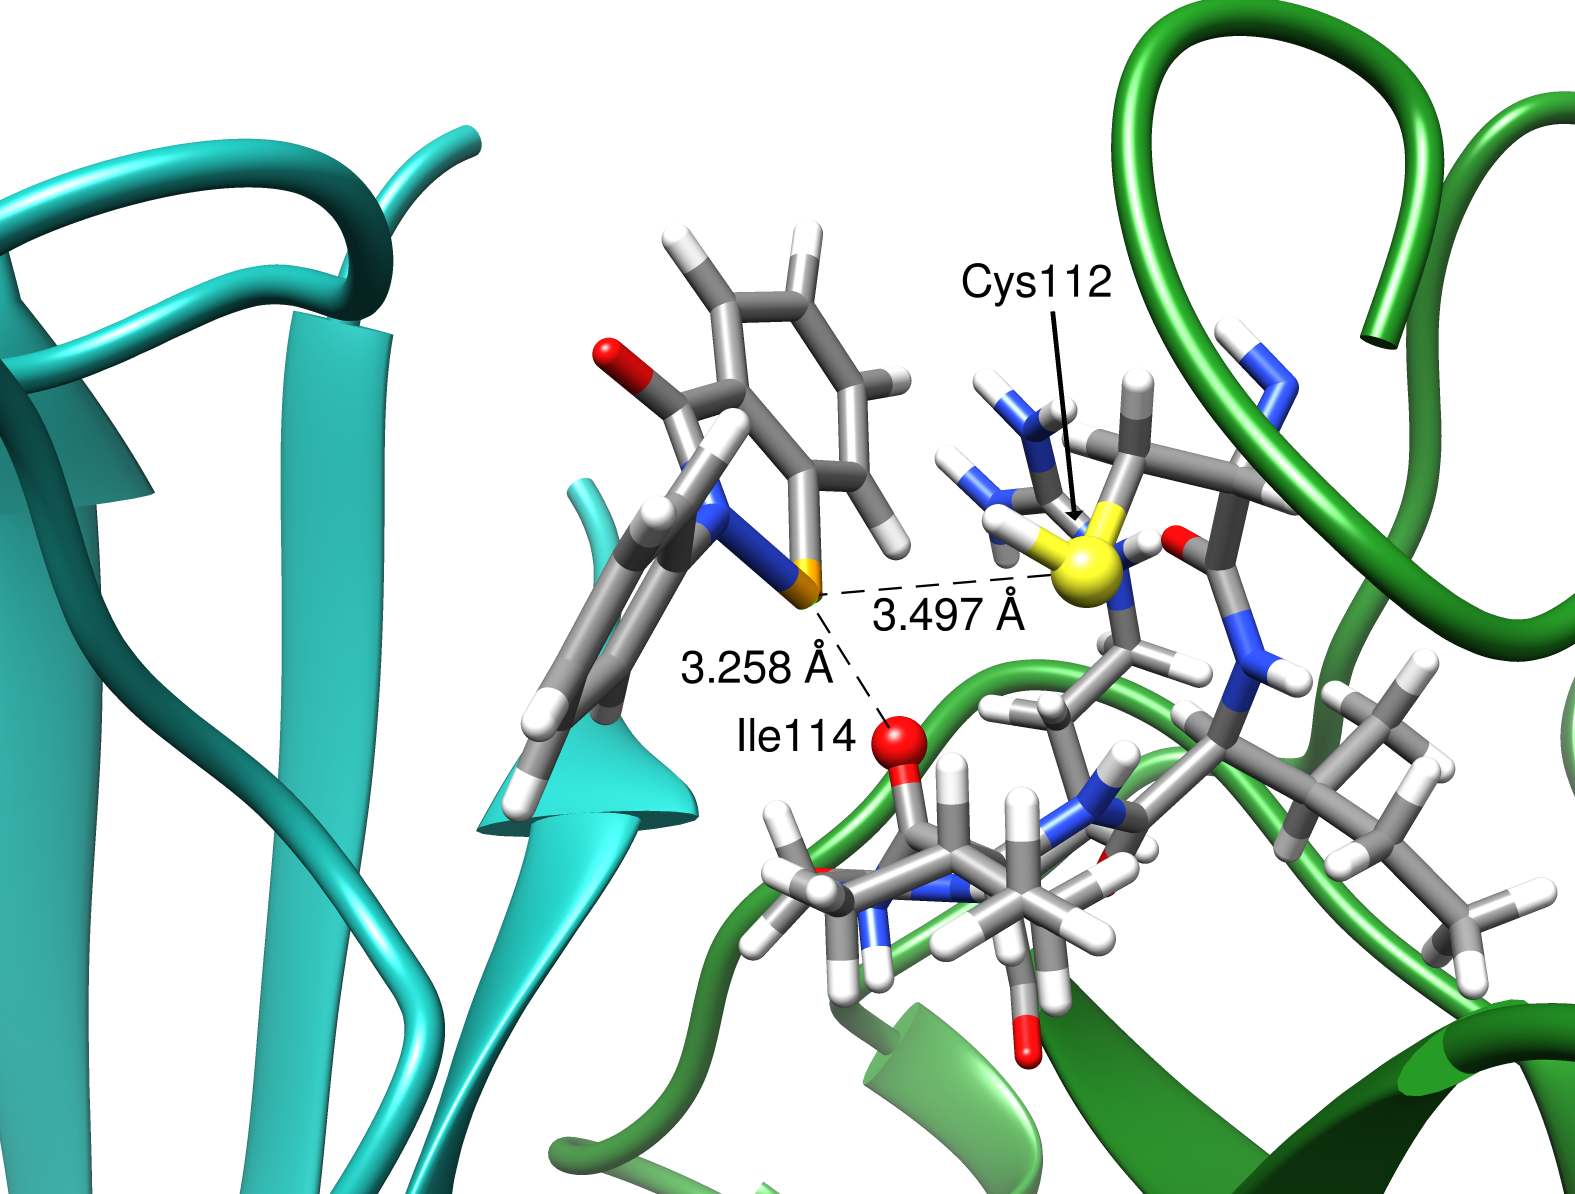
\includegraphics[width=0.75\linewidth]{Figures/bifurcated-chbond.png}
    \caption{Average binding geometry of ebselen in the SOD1 groove.}
    \label{fig:sod1-ebs}
\end{figure}

\section{Conclusion}
In conclusion, we have developed a set of parameters which can greatly improve modelling of ebselen and its derivatives.
Our model gives realistic geometries and energies of gas phase complexes, and reproduces the interaction between ebselen and a protein.
Although this work is restricted to ebselen itself, the parameters will be generally applicable to derivatives of ebselen (with appropriate charge fitting).
We hope that these results will be useful for the discovery of new targets.

\printbibliography[heading=subbibliography]
\end{refsection}
